\section{Detector}  
  
The data in these plots is the full period4 dataset unless otherwise indicated, using the files in the definition \texttt{dduenas\_pid\_testbeam\_beamlinestream\_period4\_magpol\_bug\_fix}. Selection cuts are:\\[1ex]
Pass the beamline trigger\\[1ex]
No detector deadtime\\[1ex]
Have a time-of-flight measurement\\[1ex]
Have at least one in-time detector hit.\\[1ex]

\subsection{The baby NOvA coordinates}


Figure~\ref{fig_novarot} shows the  detector rotation.

\begin{figure}[h]	   
 \centering
        	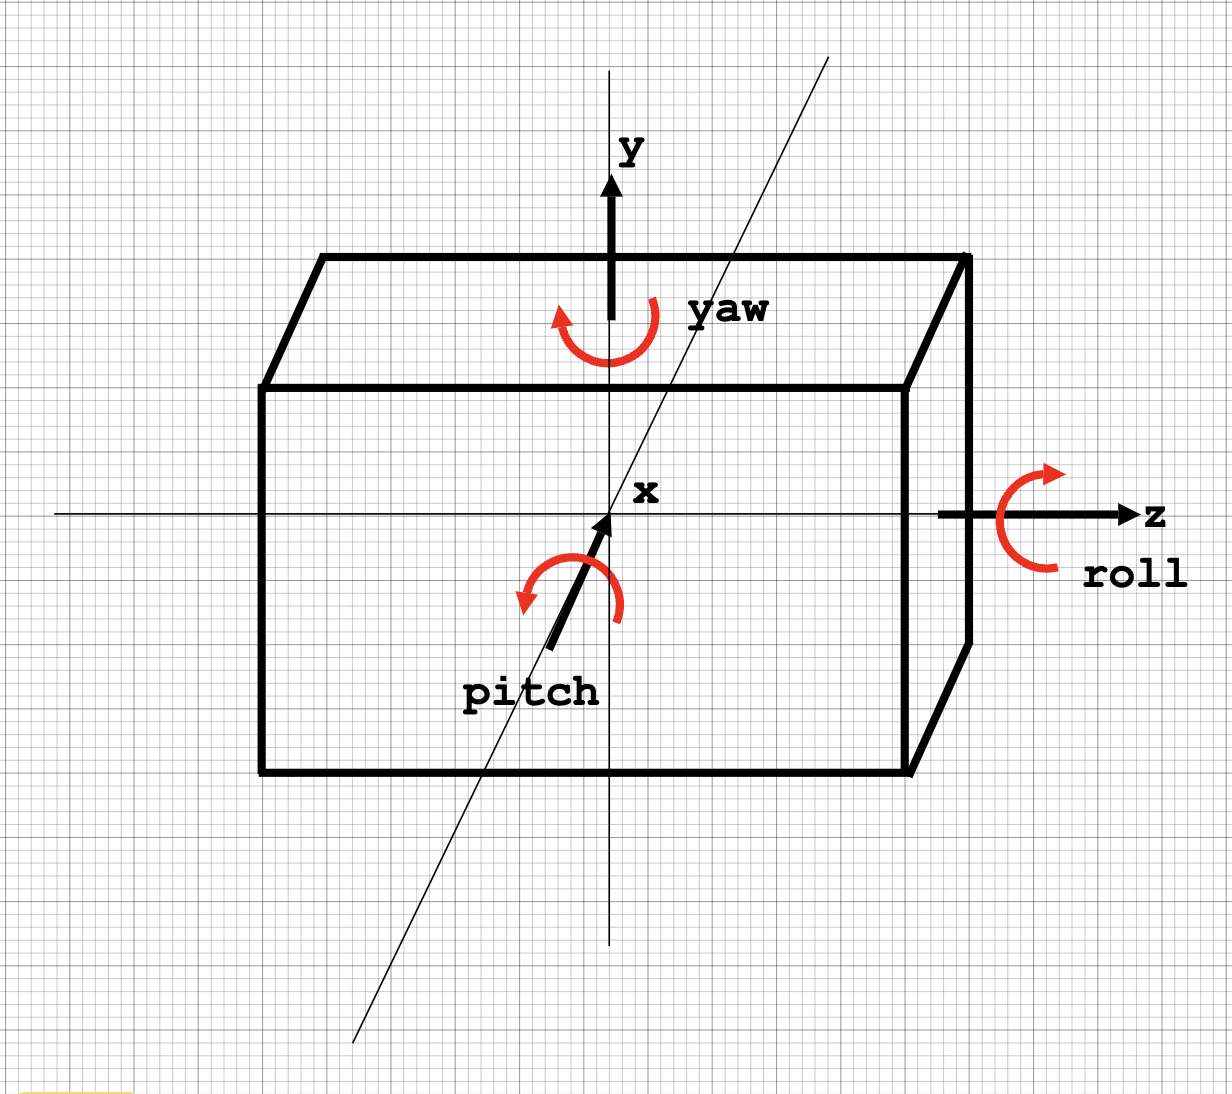
\includegraphics[scale=0.5]{novarot.png}	 
   \caption[short]{NOvA rotation.}
   \label{fig_novarot}
  \end{figure}

\subsection{Structure: Cells and Planes}
\noindent
There are 63 planes in the detector, each with 64 cells. The first plane, plane zero, has vertical cells. All the subsequent even-numbered planes have vertical cells, and the odd-numbered planes have horizontal cells. The basic geometry is as follows:\\[1ex]
The x-dimension runs east-west, from the center of cell zero at -124.706 cm to the center of cell 63 at +124.704 cm.\\
The y-dimension runs down-up, from the center of cell zero at -123.334 cm to the center of cell 63 at 126.078 cm.\\
The transverse half-width of the cells is 1.728 cm. For horizontal cells the transverse width is in y, for vertical cells it is in x.\\
The transverse half length of the cells is 130.820 cm. For horizontal cells the transverse width is in x, for vertical cells it is in y.\\
The z-dimension runs from the center of plane 0 at +3.383 cm to plane 62 at 418.033 cm. The half-depth of the cells is 2.782 cm.  \\
\noindent
The binning for the plots in this section uses the geometry considerations above, but the numbers above do not take into account the small shifts and rotations of planes with respect to one another.\\
\noindent
Each plane is slightly rotated around the z-axis with respect to the superblock. This is just a fact of life, not something that was done deliberately. The rotations can be seen in Figure~\ref{fig_dethit_plane01}  for the first two planes, with the remaining plots available in Appendix~\ref{app_fit_XY}  . A straight line fit provides the slope $m$ and the angle is $\theta= \arctan(m)$. The angles have been checked against those in the testbeam survey \href{https://github.com/novaexperiment/novasoft/blob/main/Geometry/gdml/tbscripts/tb_survey.txt}{the testbeam survey} and are in agreement.  Figure~\ref{fig_detxz} shows the transverse position of cell hits as a function of z.  
  



 \begin{figure}	   
 \centering
        	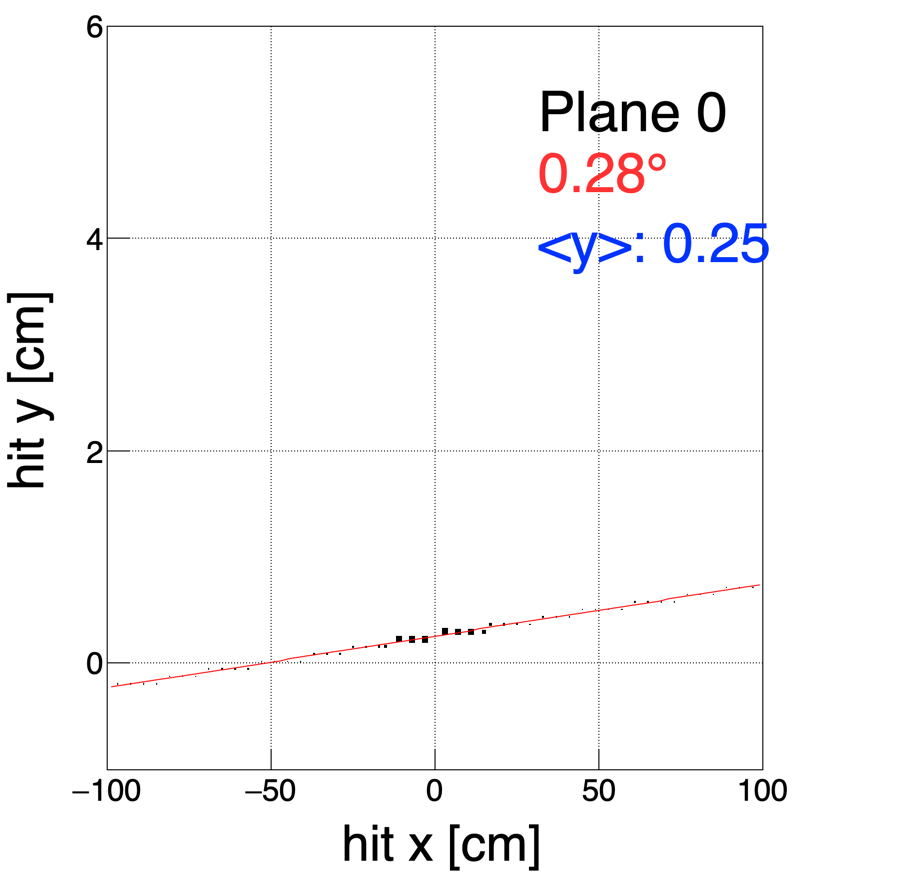
\includegraphics[scale=0.25]{det_xy_pol-1_period4_miss0_plane0.png}
	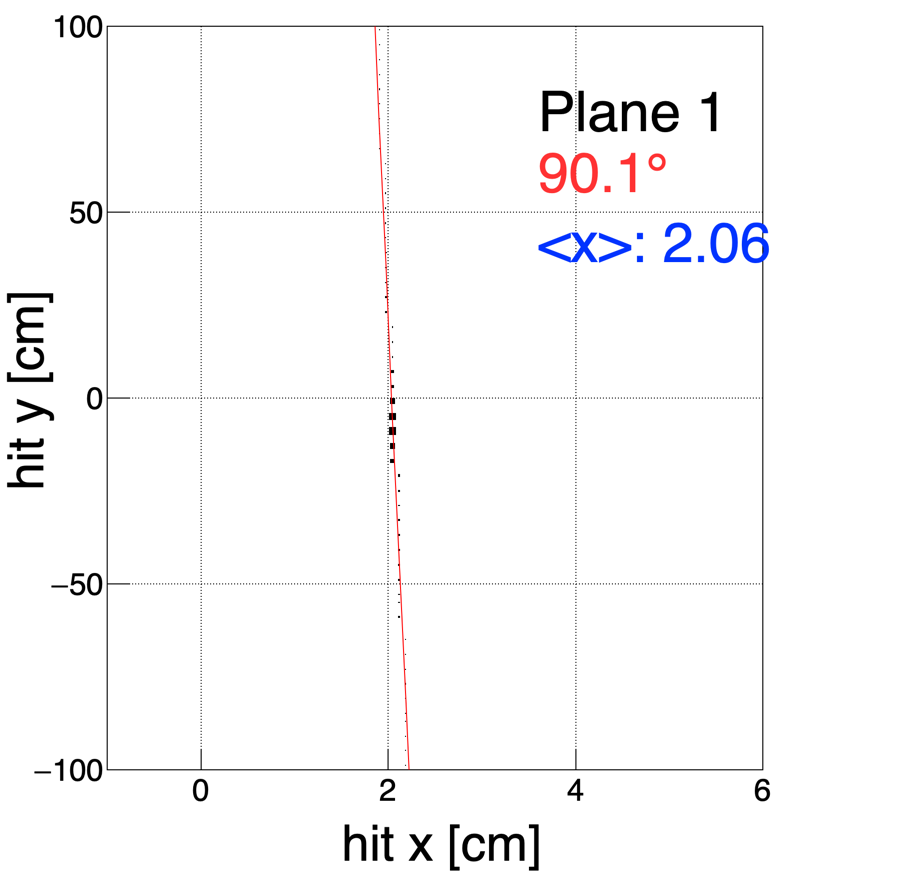
\includegraphics[scale=0.25]{det_xy_pol-1_period4_miss0_plane1.png}
		 \caption{The xy positions of hits in (left) plane 0 and (right) plane 1. Plots made using the script \texttt{single-plot-detxy.py}.}	
   \label{fig_dethit_plane01}
  \end{figure}

 \begin{figure}	   
 \centering
  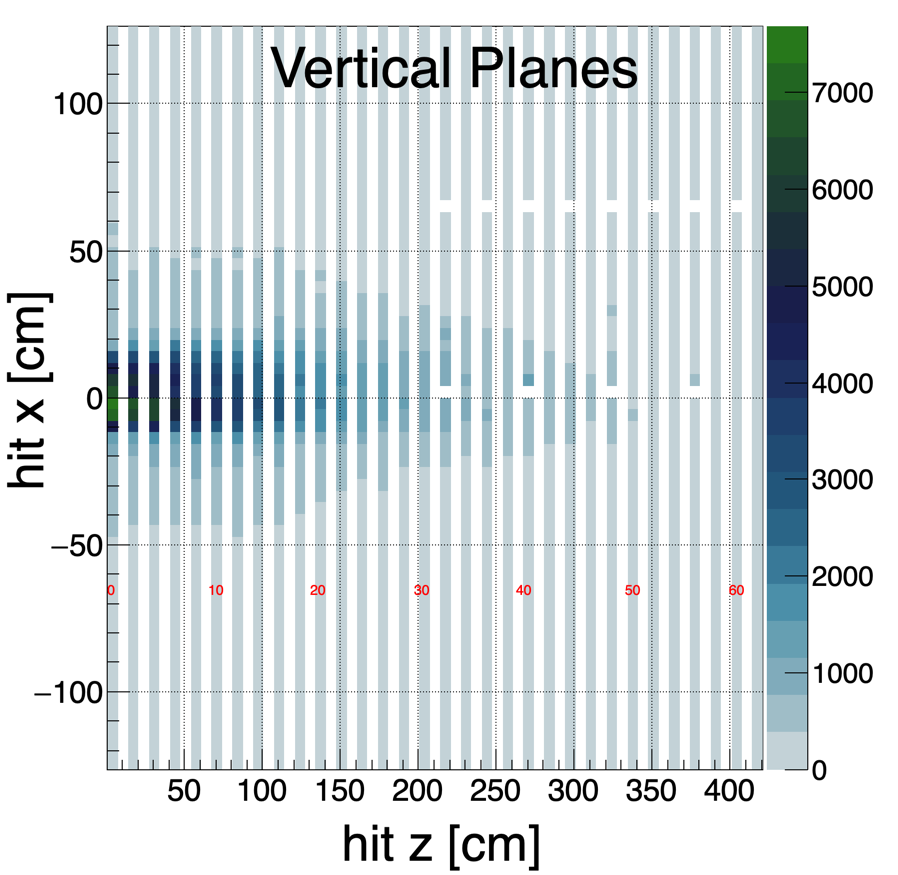
\includegraphics[scale=0.25]{det_xzdetail_pol-1_period4_miss0.png}
   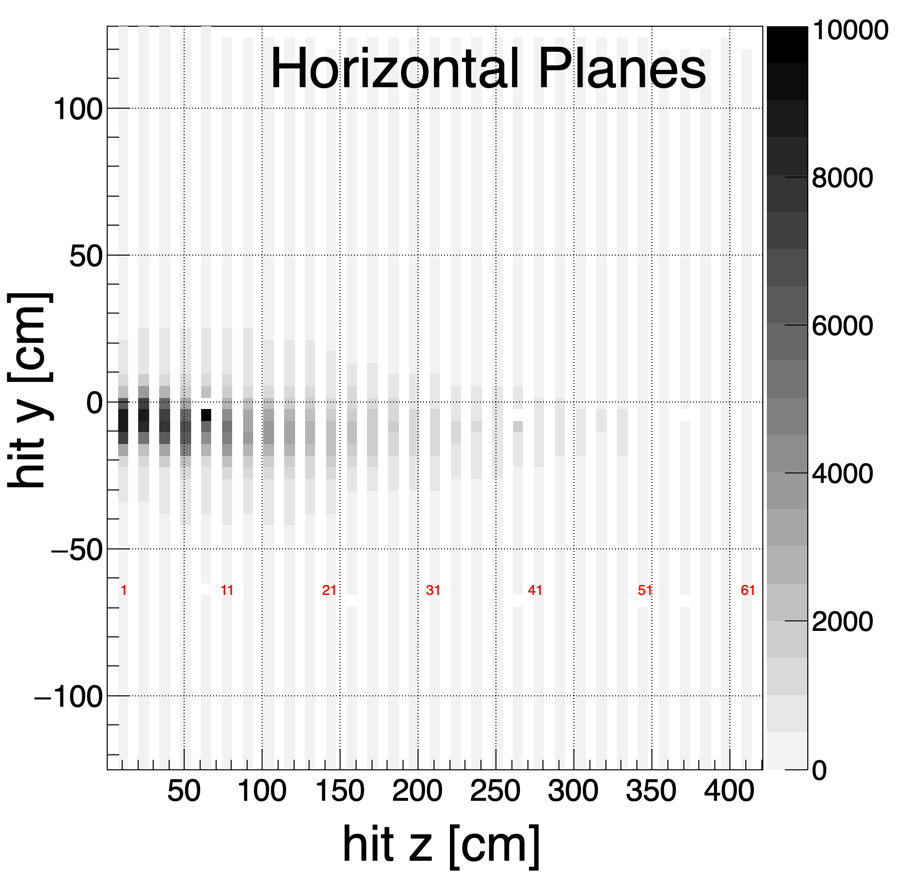
\includegraphics[scale=0.25]{det_yzdetail_pol-1_period4_miss0.png}
  \caption{Detector cell hit z,x (left) and z,y (right) positions. There are a few empty bins which is just a result of the imperfect binning described in the text.
  Scripts are \texttt{single-plot-detxzdetail.py} and \texttt{single-plot-detyzdetail.py}  }			
   \label{fig_detxz}
  \end{figure}
  
  

\noindent
The energy deposited in calorimeter cells is recorded as PE (PhotoElectrons) and the calibration then converts this into a proper energy measurement in GeV. Figure~\ref{fig_calibhits0} shows the before and after of this process for hits in plane 0 of the detector. The cells in plane 0 (and all subsequent even-numbered planes) are vertical, such that only a measurement of the x-position of a cell can be known. Figure~\ref{fig_calibhits1} shows hits in plane 1 of the detector.  The calibration fails in plane 1 (and all subsequent odd-numbered planes) because the horizontal cells were under-filled with scintillator early on in data taking, and this made it into the simulation. \textcolor{red}{Watch this space for updated plots with Robert's new calibration}.  These plots are available for every plane in Appendix ~\ref{app_PE_XY}.  Figure~\ref{fig_detenergyz} shows energy deposited as a function of z for uncalibrated and calibrated cell hit energies. 


 \begin{figure}	   
 \centering
  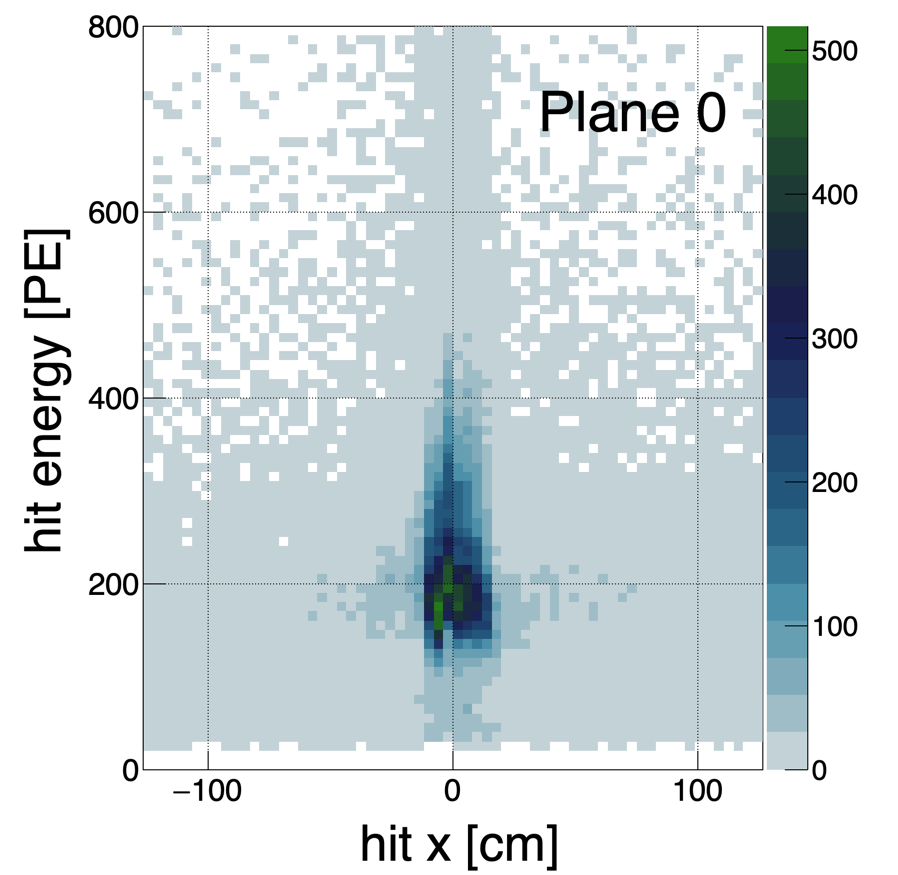
\includegraphics[scale=0.25]{det_xype_pol-1_period4_miss0_plane0.png}
   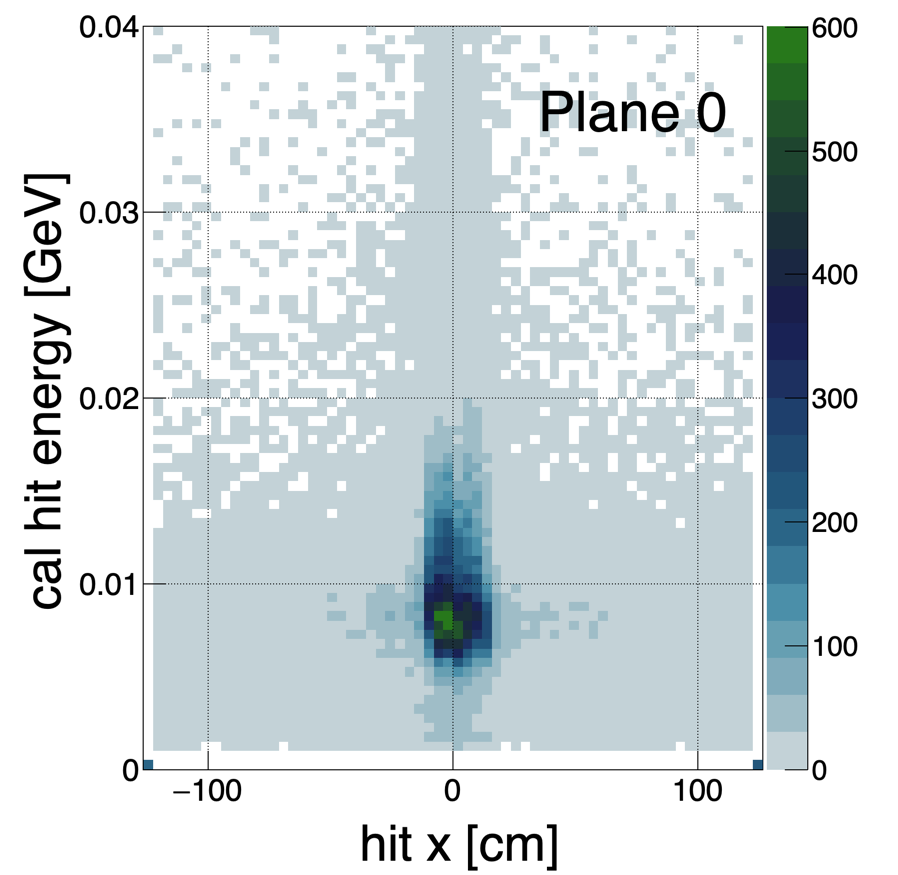
\includegraphics[scale=0.25]{det_xygev_pol-1_period4_miss0_plane0.png}
  \caption{Plane 0 hit energies as a function of the cell positions within the detector for (left) uncalibrated hits and (right) calibrated hits. Scripts are single-plot-detxpe.py and single-plot-detxgev.py.}			
   \label{fig_calibhits0}
  \end{figure}
%
%  
% 
% 
  \begin{figure}	   
 \centering
  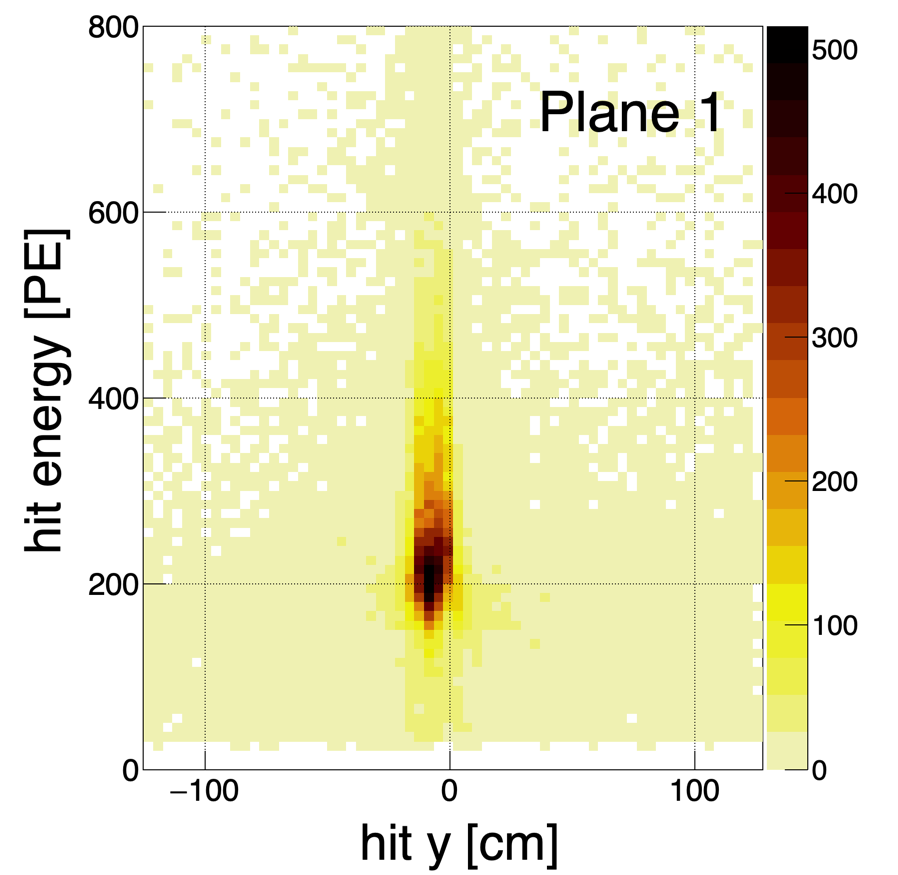
\includegraphics[scale=0.25]{det_xype_pol-1_period4_miss0_plane1.png}
   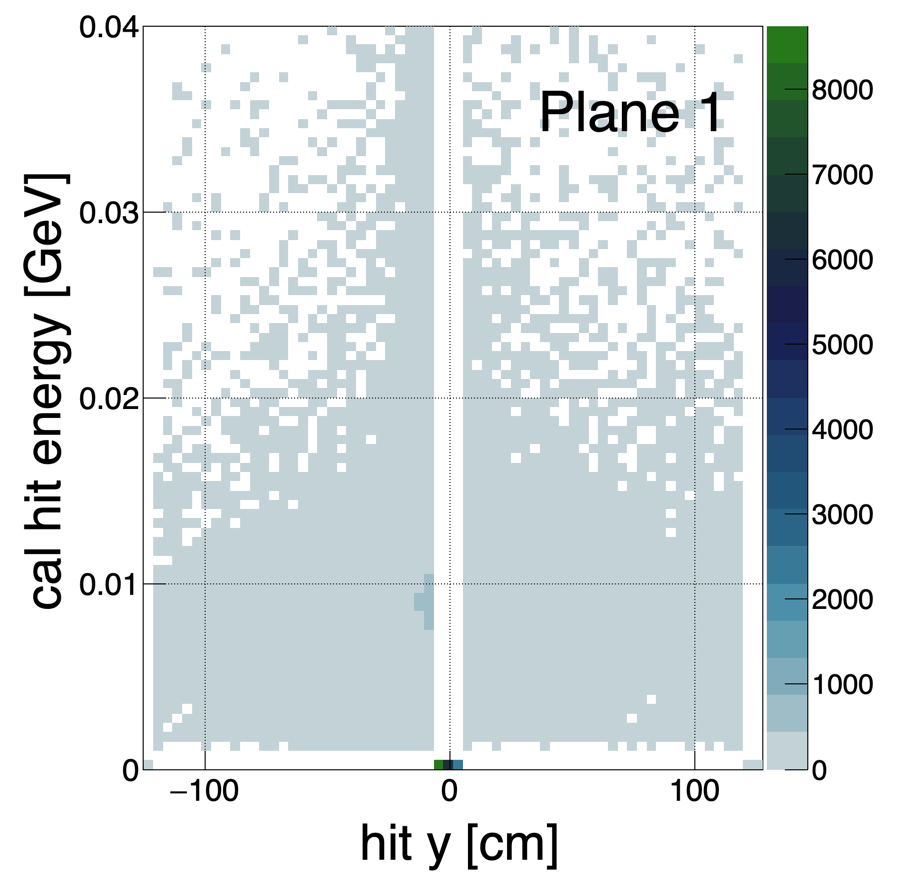
\includegraphics[scale=0.25]{det_xygev_pol-1_period4_miss0_plane1.png}
  \caption{Plane 1 hit energies as a function of the cell positions within the detector for (left) uncalibrated hits and (right) calibrated hits.}			
   \label{fig_calibhits1}
  \end{figure}


 \begin{figure}	   
 \centering
  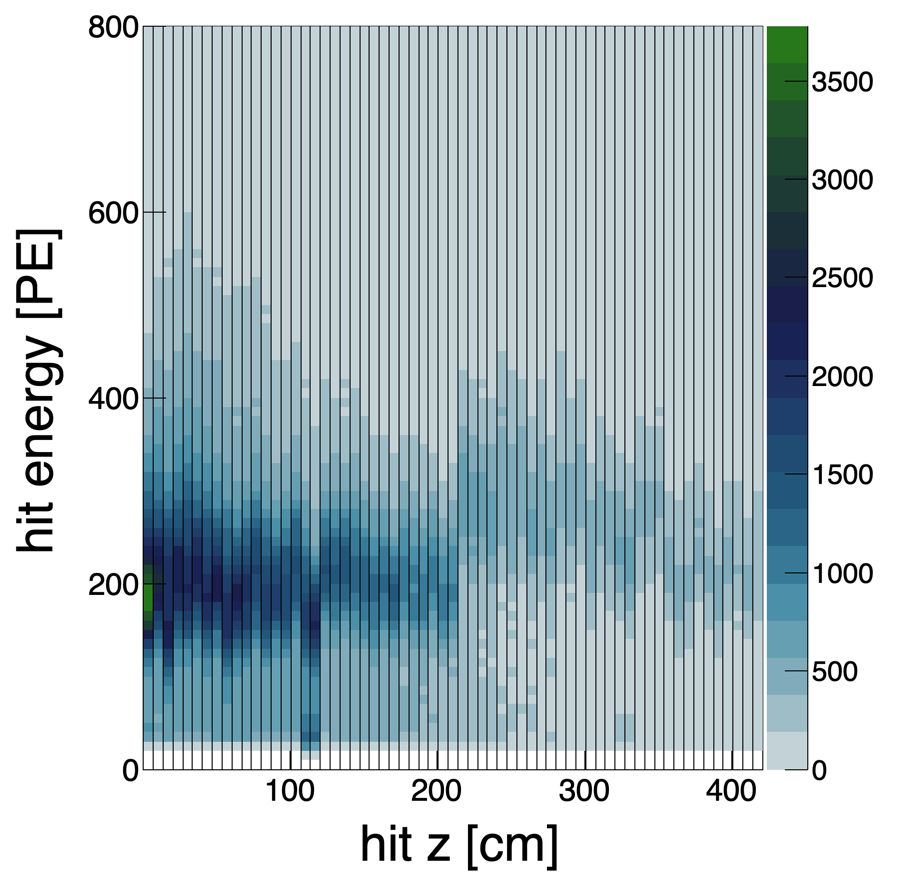
\includegraphics[scale=0.25]{det_pezdetail_pol-1_period4_miss0.png}
   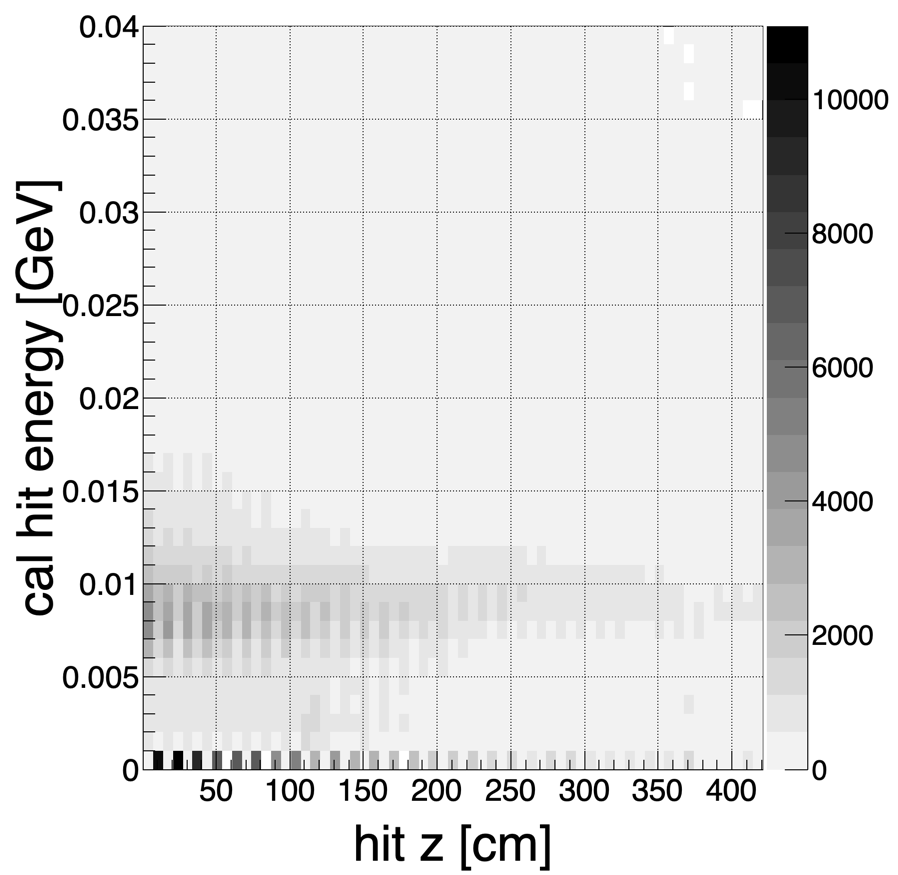
\includegraphics[scale=0.25]{det_gevzdetail_pol-1_period4_miss0.png}
  \caption{Detector cell hit energy (left) before and (right) after calibration.}			
   \label{fig_detenergyz}
  \end{figure}
%  

   \begin{figure}	   
 \centering
  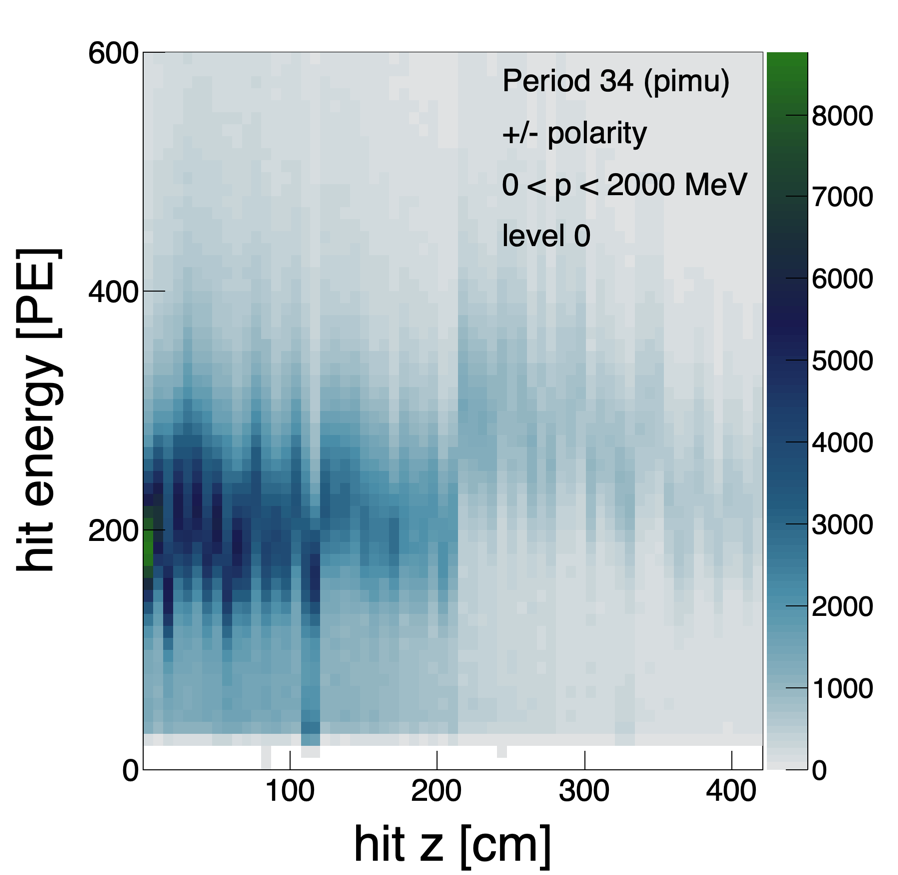
\includegraphics[scale=0.25]{pimu_34_hitz_hitpe_level0_posneg_AllMom_Cur1.png}
   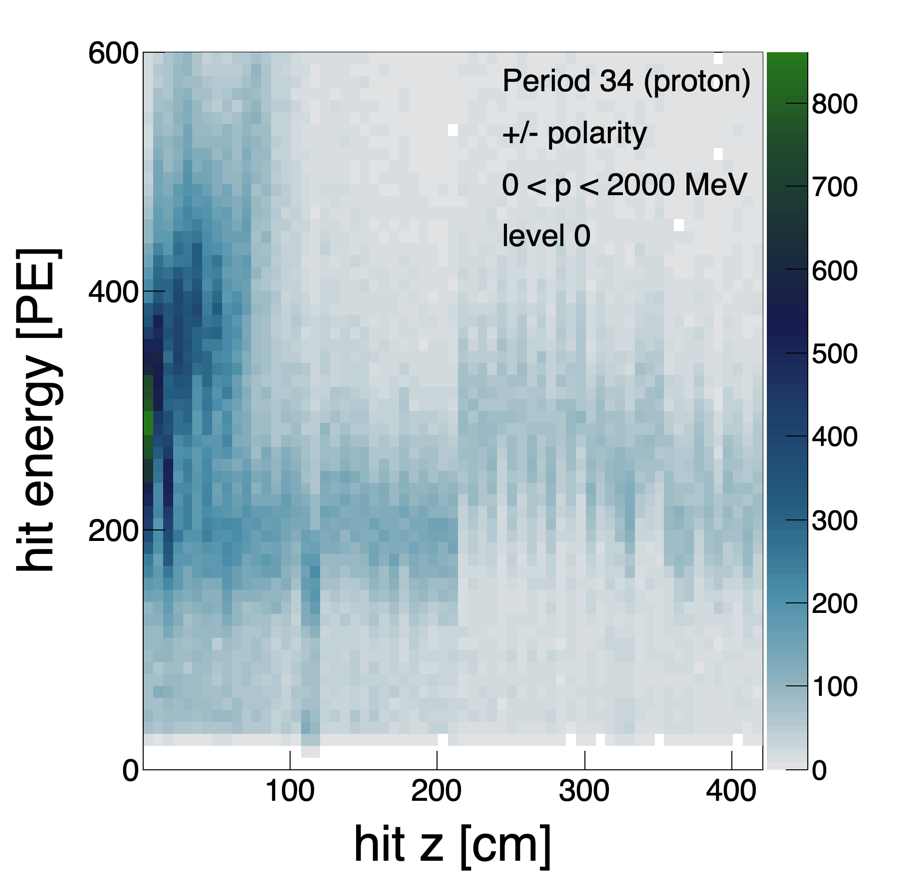
\includegraphics[scale=0.25]{proton_34_hitz_hitpe_level0_posneg_AllMom_Cur1.png}
     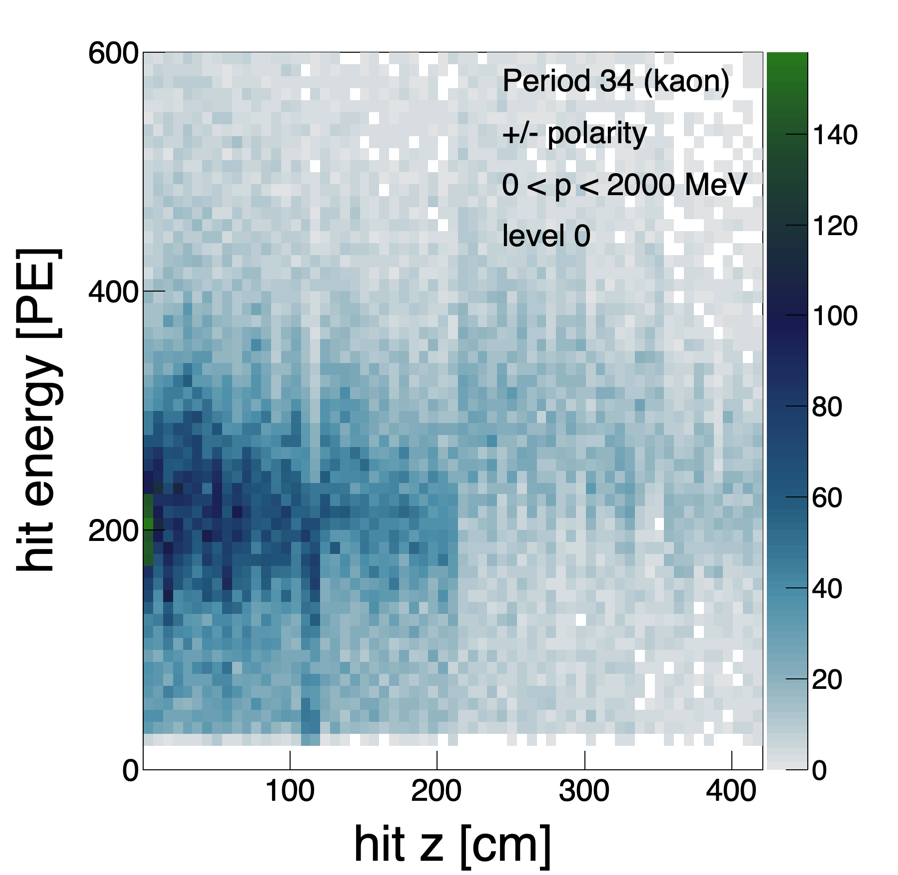
\includegraphics[scale=0.25]{kaon_34_hitz_hitpe_level0_posneg_AllMom_Cur1.png}
   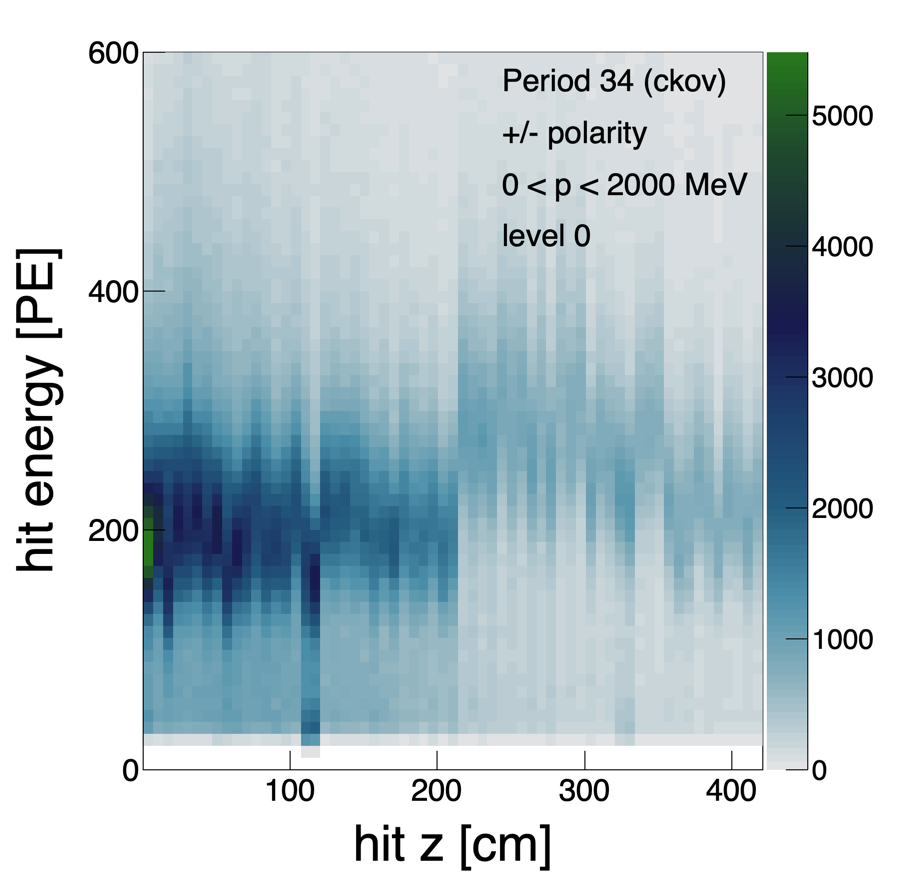
\includegraphics[scale=0.25]{ckov_34_hitz_hitpe_level0_posneg_AllMom_Cur1.png}
     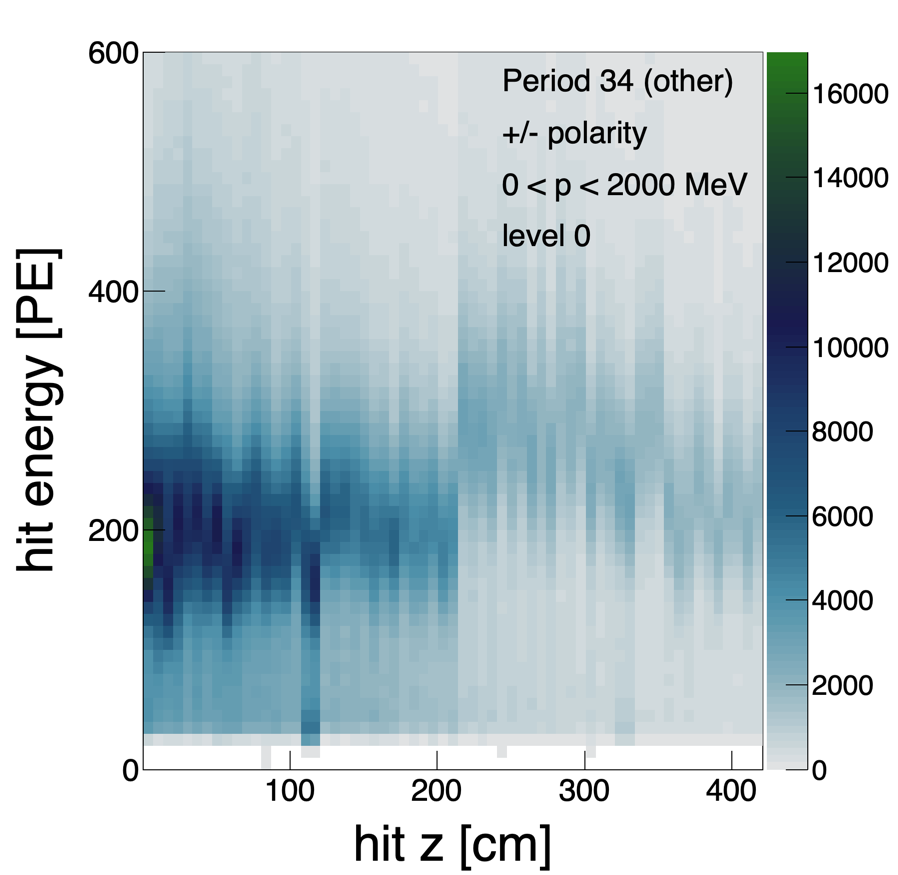
\includegraphics[scale=0.25]{other_34_hitz_hitpe_level0_posneg_AllMom_Cur1.png}

  \caption{Hit Pe versus average z for different particles - script 2d-plot-style.py.}			
   \label{fig_pez}
  \end{figure}
%    
\subsection{Hit properties}

Cell hits that are in time with the trigger can be matched to a beamline track (with ``known'' particle type). Here are some plots of some hit properties. 


 \begin{figure}	   
 \centering
  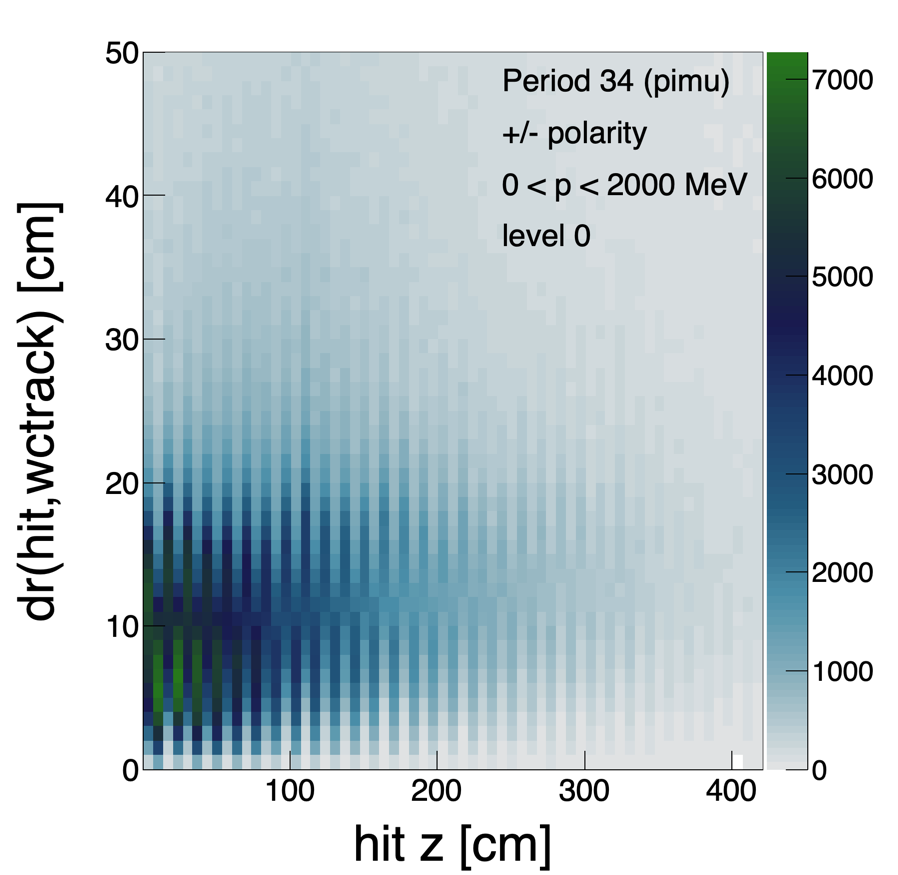
\includegraphics[scale=0.25]{pimu_34_hitz_hitdr_level0_posneg_AllMom_Cur1.png}
   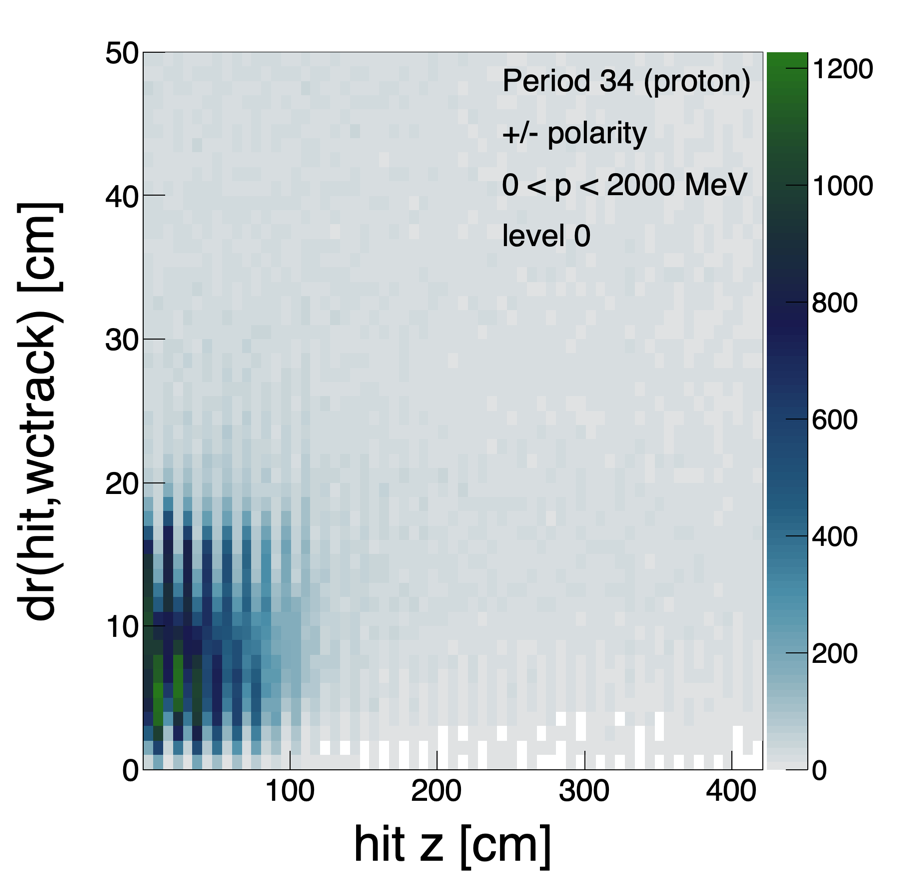
\includegraphics[scale=0.25]{proton_34_hitz_hitdr_level0_posneg_AllMom_Cur1.png}
     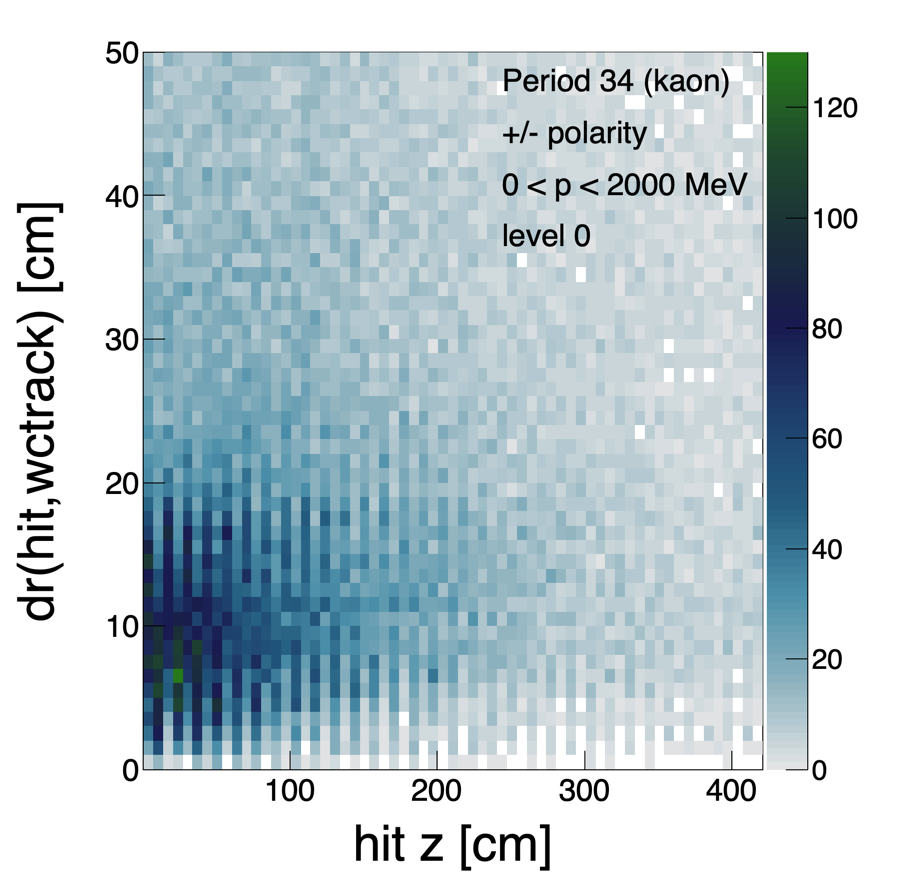
\includegraphics[scale=0.25]{kaon_34_hitz_hitdr_level0_posneg_AllMom_Cur1.png}
   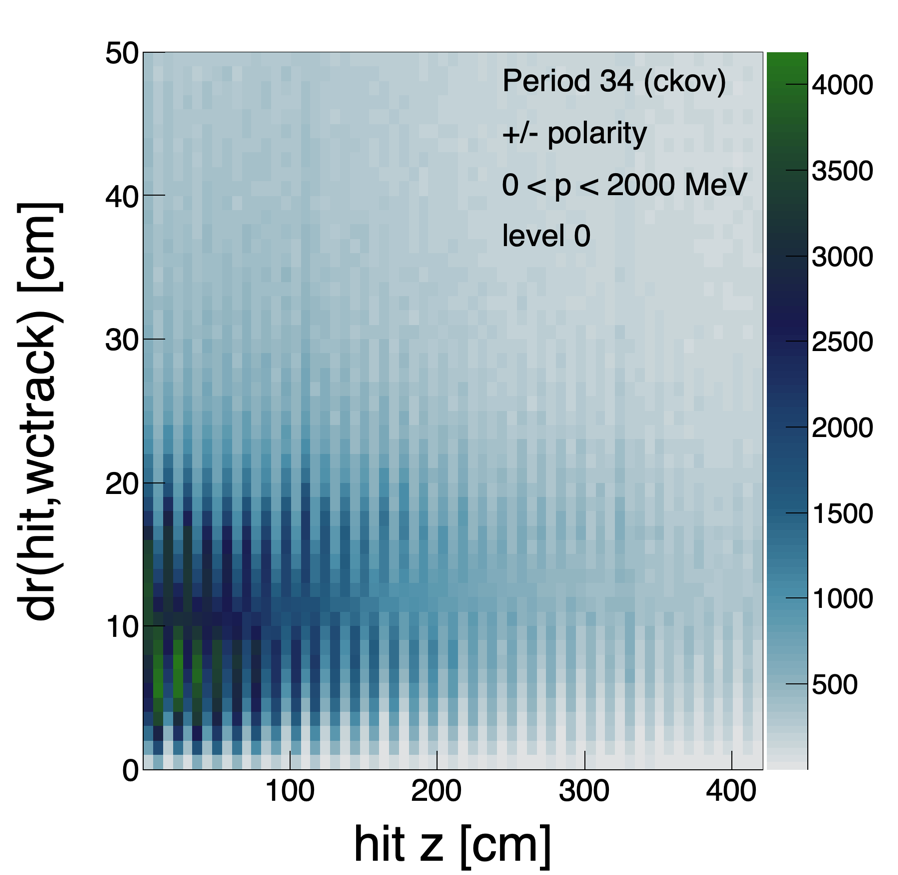
\includegraphics[scale=0.25]{ckov_34_hitz_hitdr_level0_posneg_AllMom_Cur1.png}
     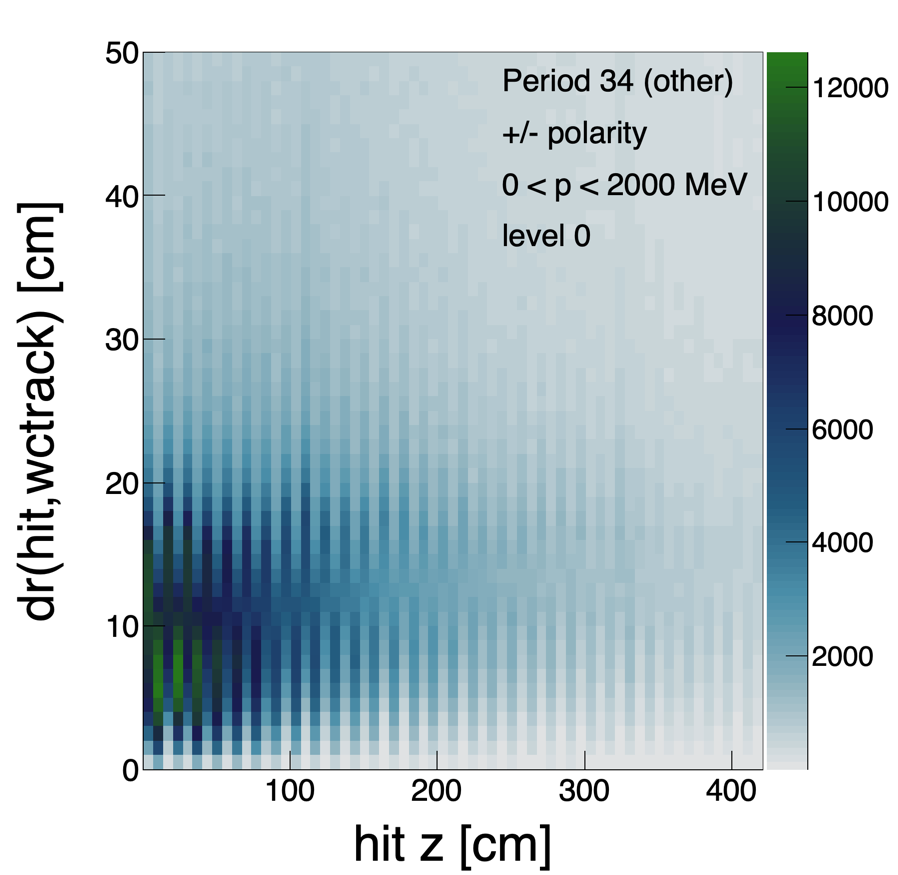
\includegraphics[scale=0.25]{other_34_hitz_hitdr_level0_posneg_AllMom_Cur1.png}

  \caption{Drs - script single-plot-detdrzdetail.py.}			
   \label{fig_detdrz}
  \end{figure}
  
   \begin{figure}	   
 \centering
  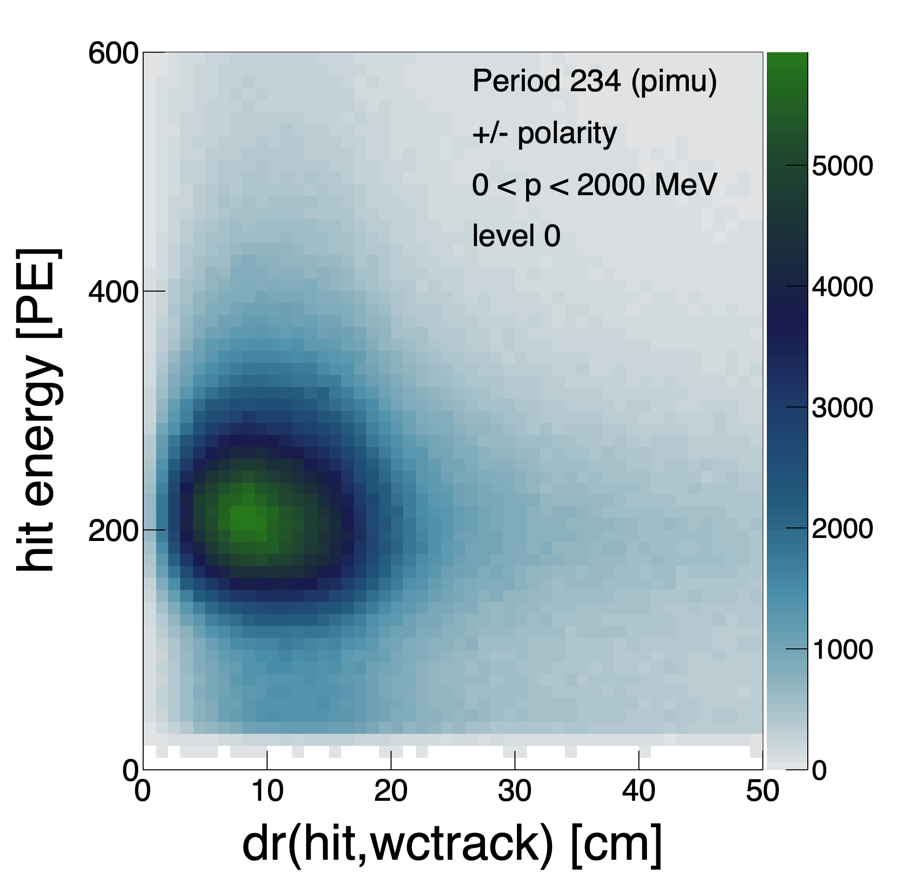
\includegraphics[scale=0.25]{pimu_234_hitdr_hitpe_level0_posneg_AllMom_Cur1.png}
   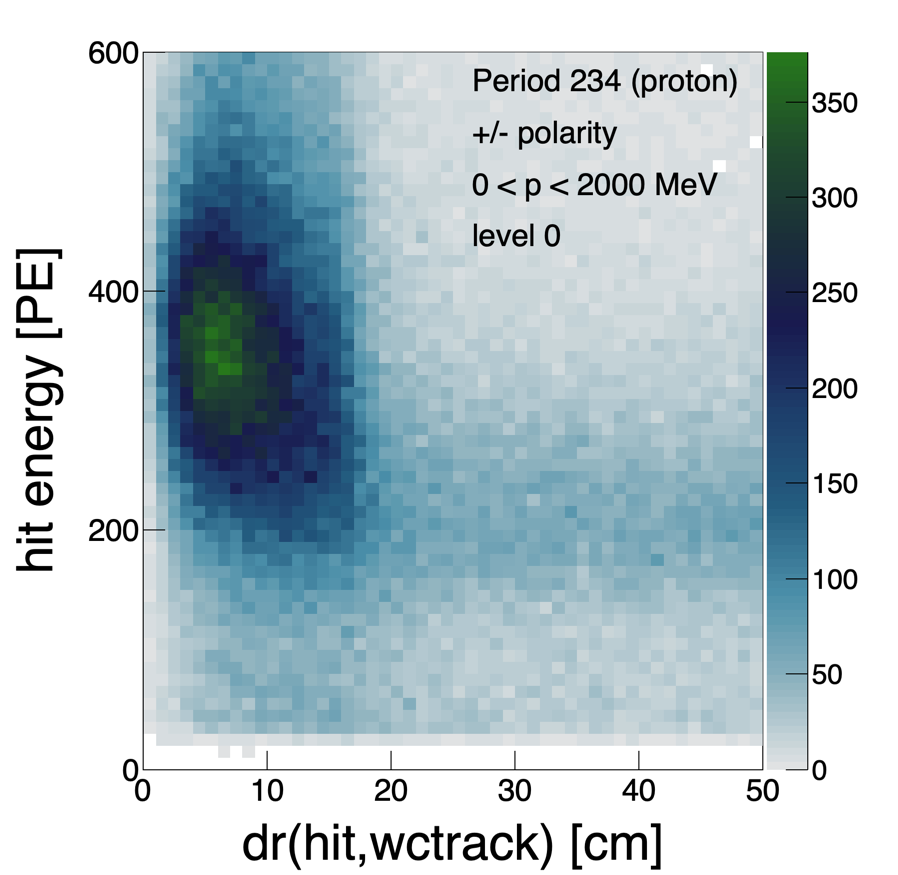
\includegraphics[scale=0.25]{proton_234_hitdr_hitpe_level0_posneg_AllMom_Cur1.png}
     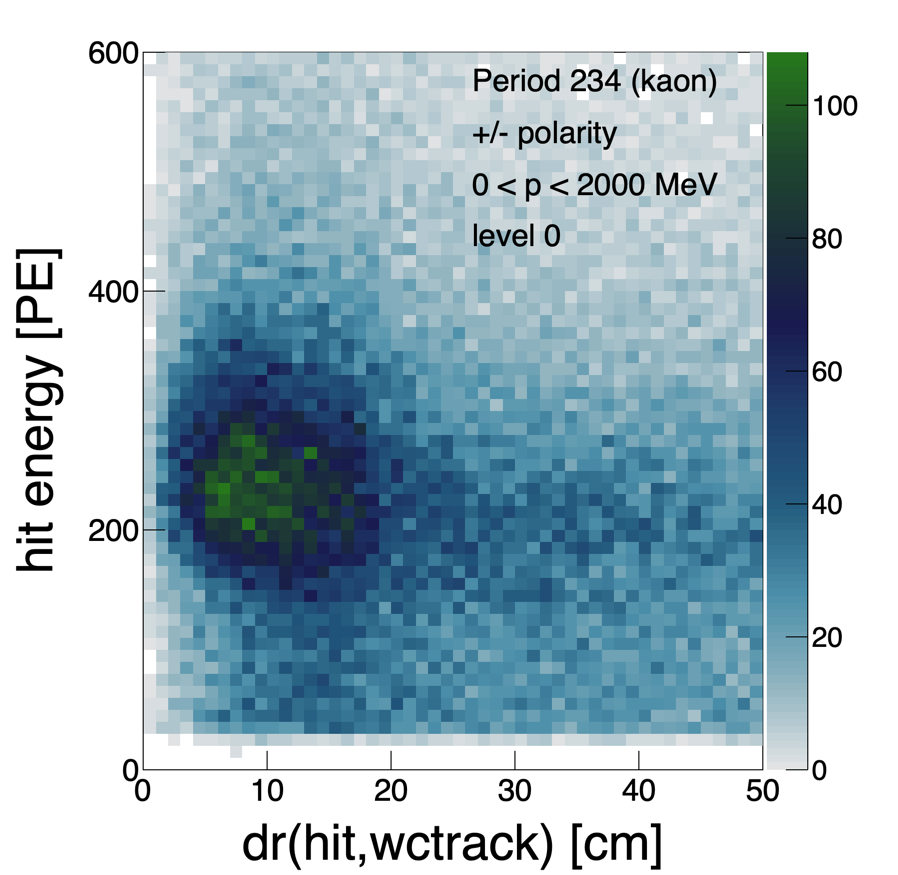
\includegraphics[scale=0.25]{kaon_234_hitdr_hitpe_level0_posneg_AllMom_Cur1.png}
   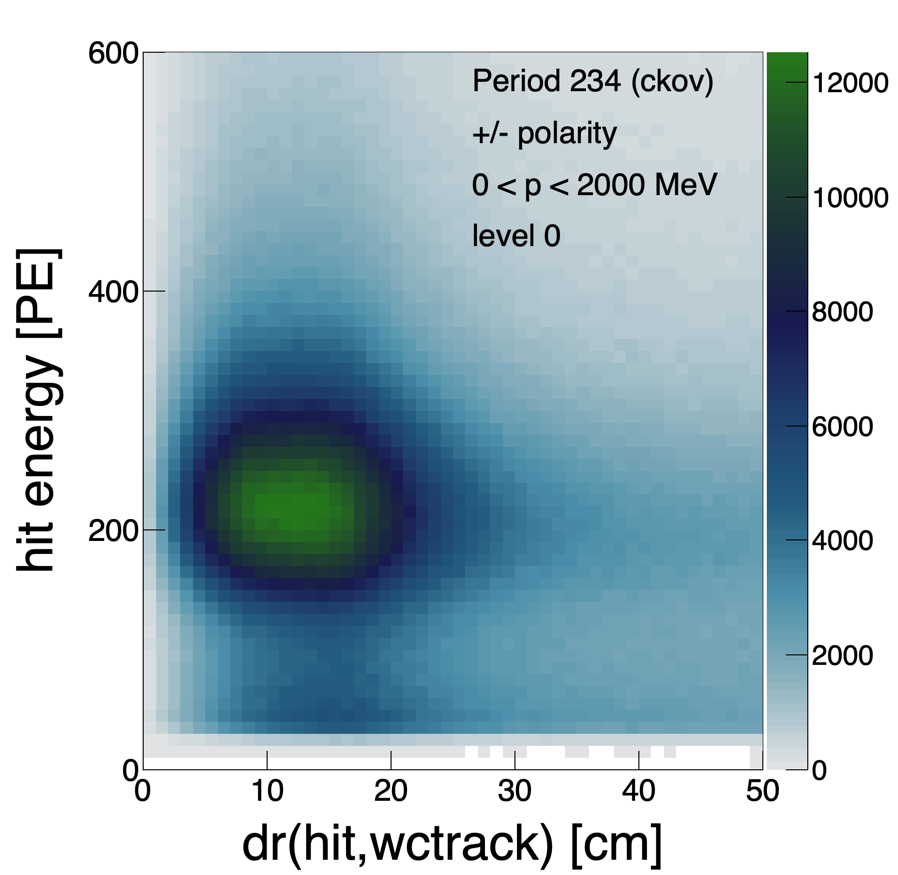
\includegraphics[scale=0.25]{ckov_234_hitdr_hitpe_level0_posneg_AllMom_Cur1.png}
     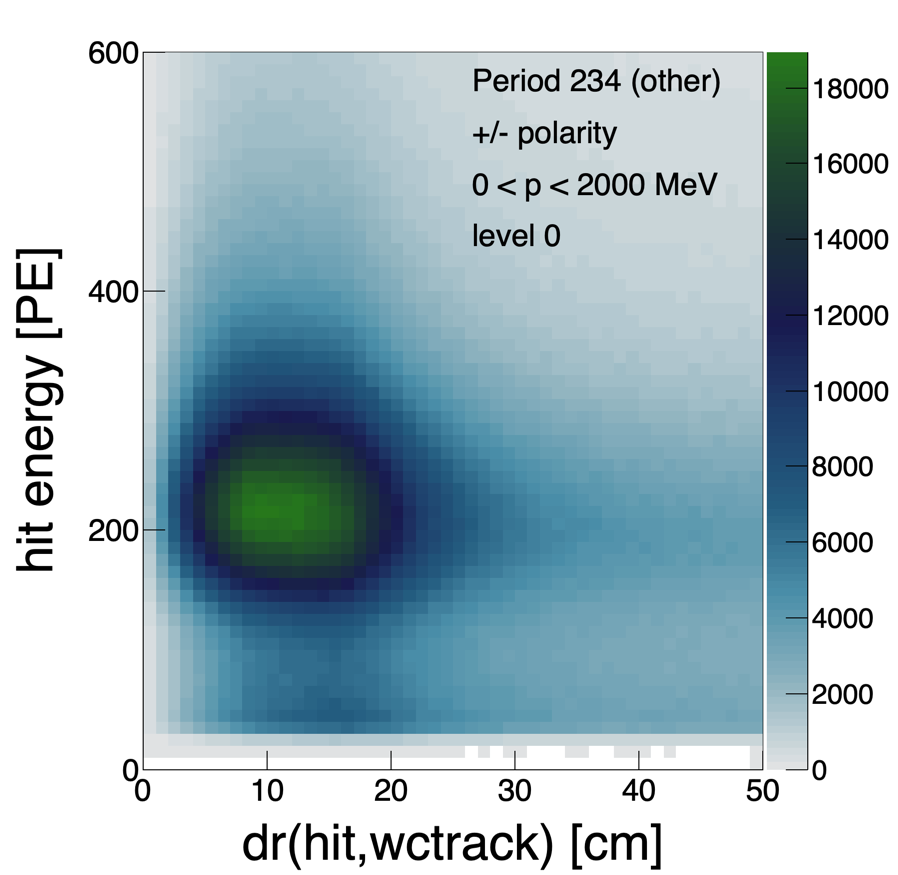
\includegraphics[scale=0.25]{other_234_hitdr_hitpe_level0_posneg_AllMom_Cur1.png}

  \caption{Dr versus PE - script 2d-plot-style.py.}			
   \label{fig_detdrpe}
  \end{figure}

   \begin{figure}	   
 \centering
  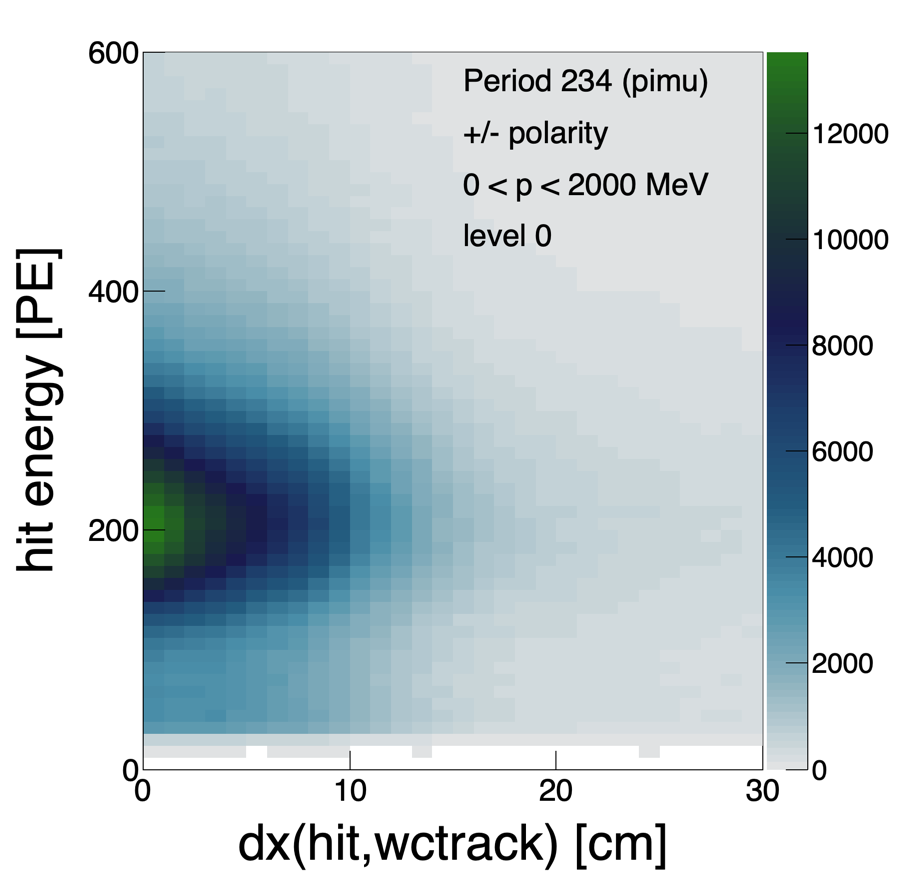
\includegraphics[scale=0.25]{pimu_234_hitdx_hitpe_level0_posneg_AllMom_Cur1.png}
   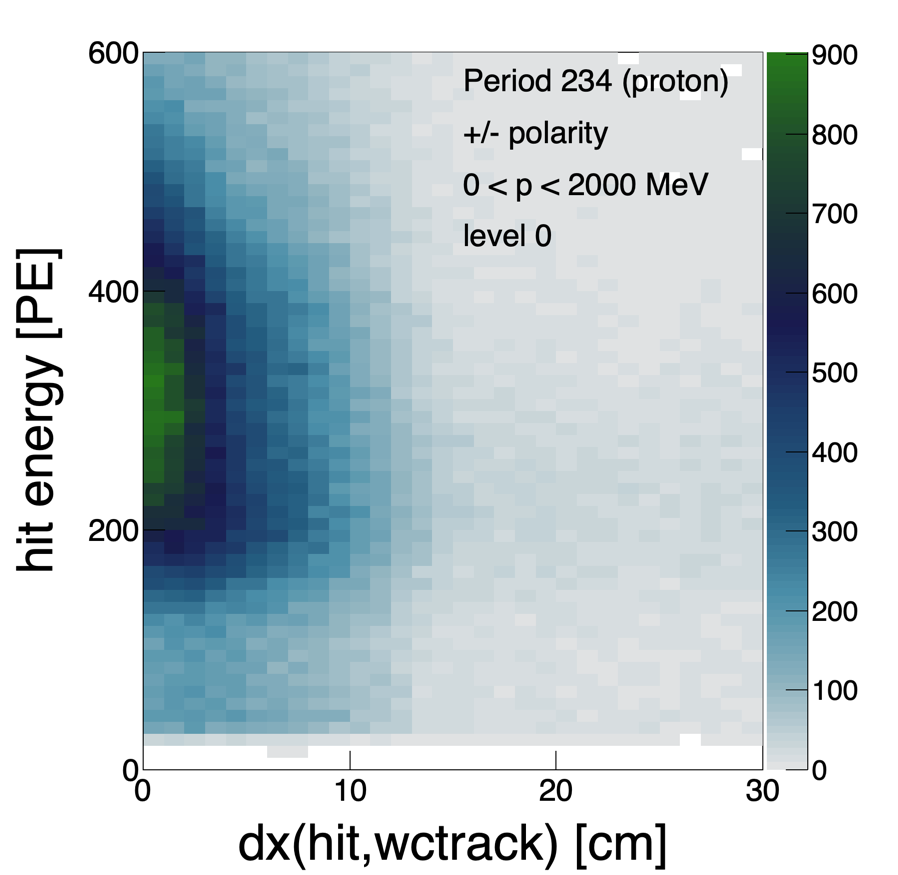
\includegraphics[scale=0.25]{proton_234_hitdx_hitpe_level0_posneg_AllMom_Cur1.png}
     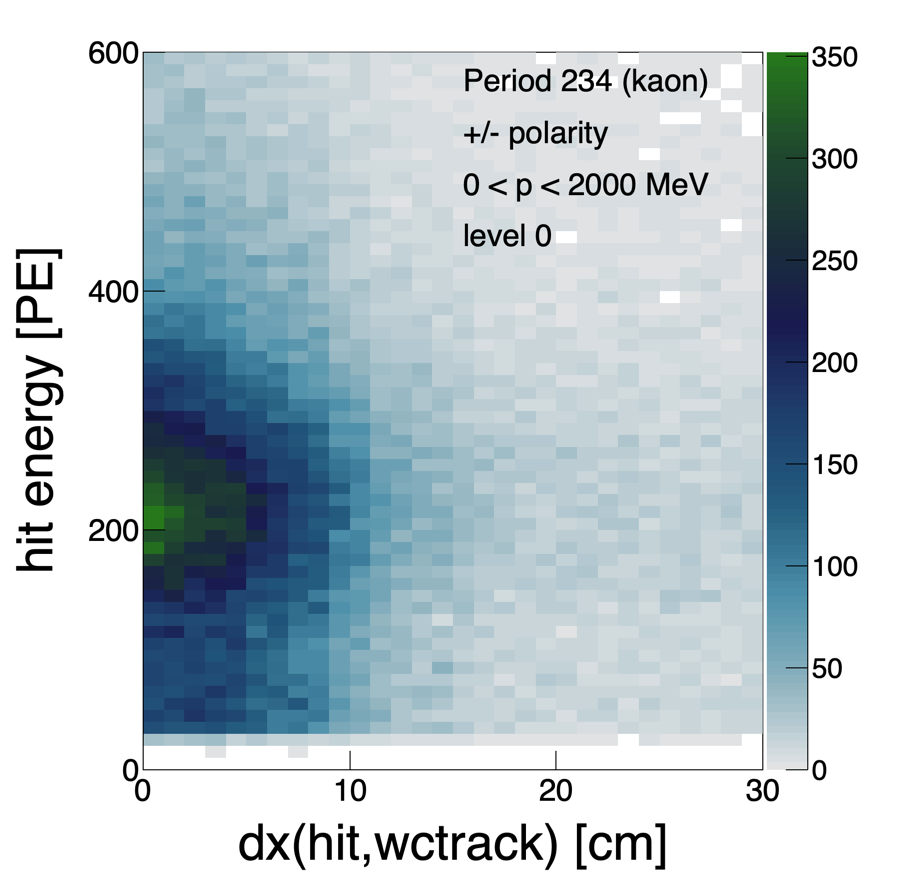
\includegraphics[scale=0.25]{kaon_234_hitdx_hitpe_level0_posneg_AllMom_Cur1.png}
   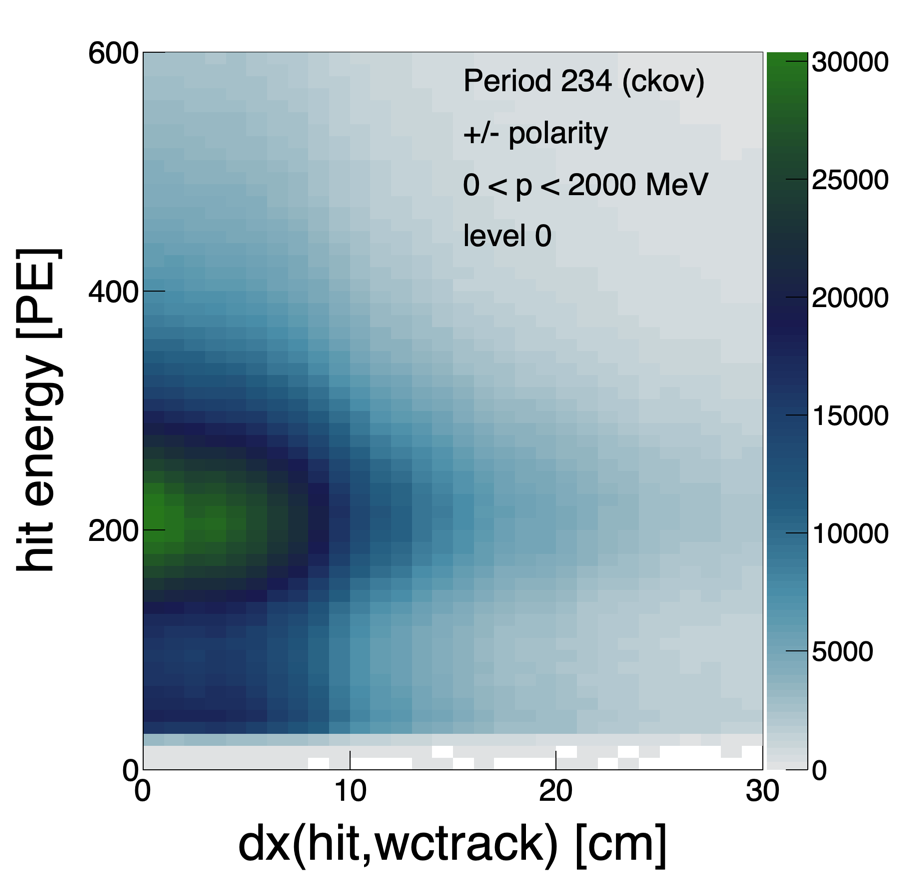
\includegraphics[scale=0.25]{ckov_234_hitdx_hitpe_level0_posneg_AllMom_Cur1.png}
     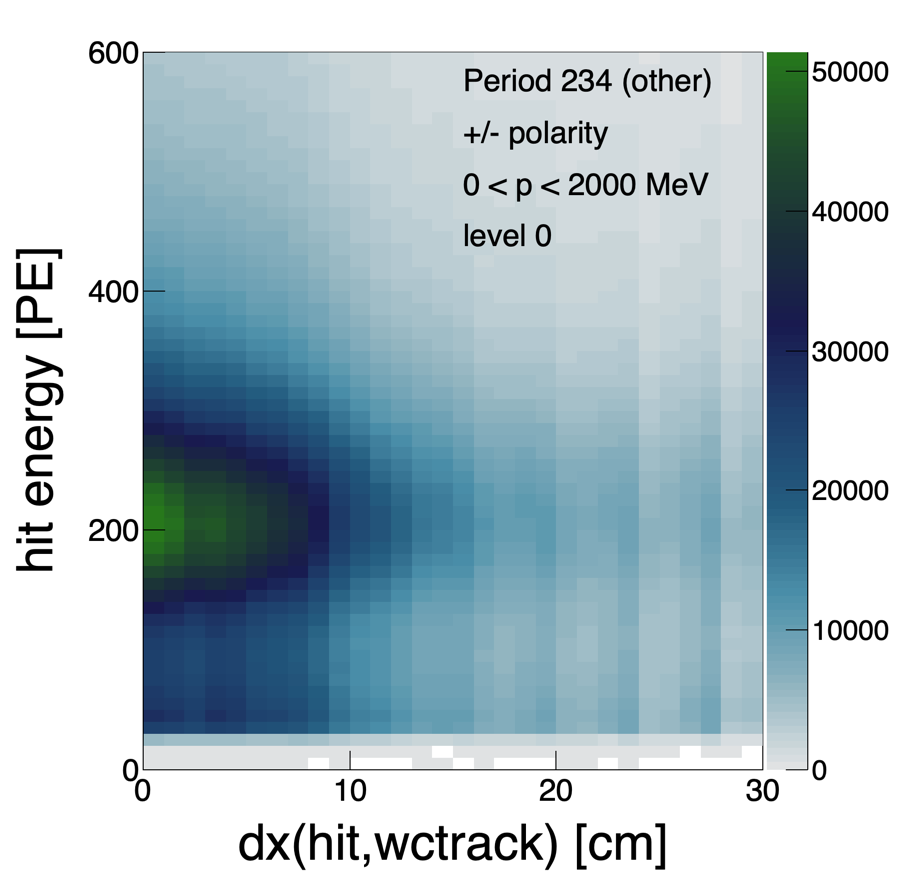
\includegraphics[scale=0.25]{other_234_hitdx_hitpe_level0_posneg_AllMom_Cur1.png}

  \caption{Dx versus PE - script 2d-plot-style.py.}			
   \label{fig_detdxpe}
  \end{figure}
  

   \begin{figure}	   
 \centering
  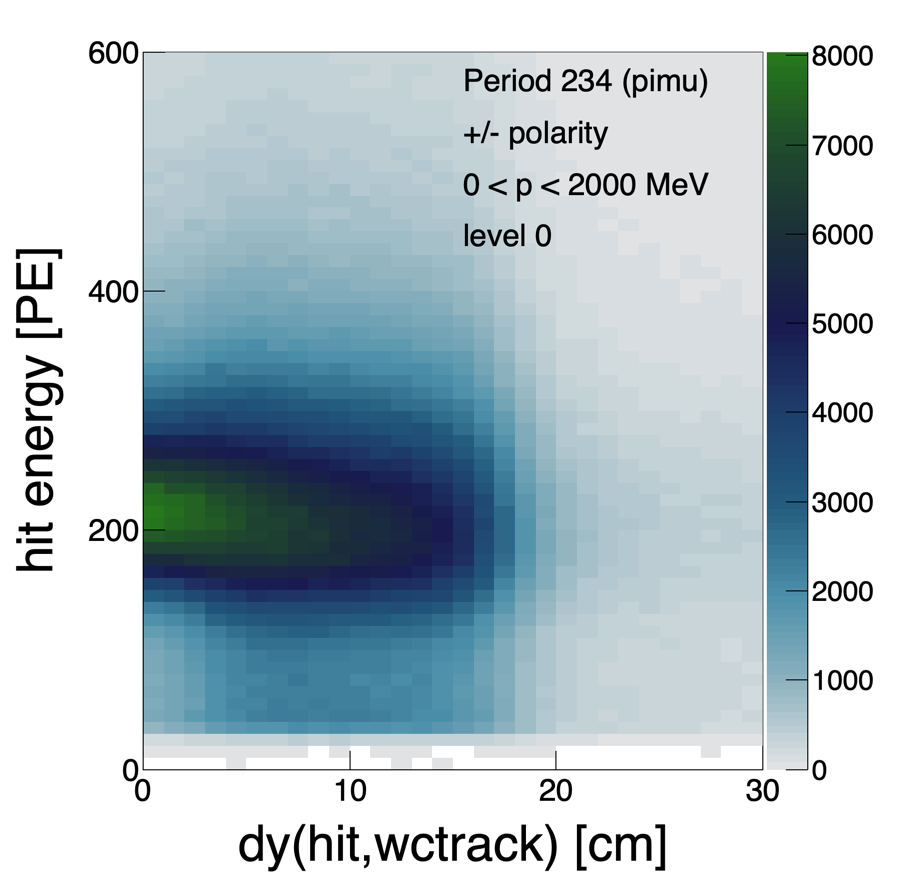
\includegraphics[scale=0.25]{pimu_234_hitdy_hitpe_level0_posneg_AllMom_Cur1.png}
   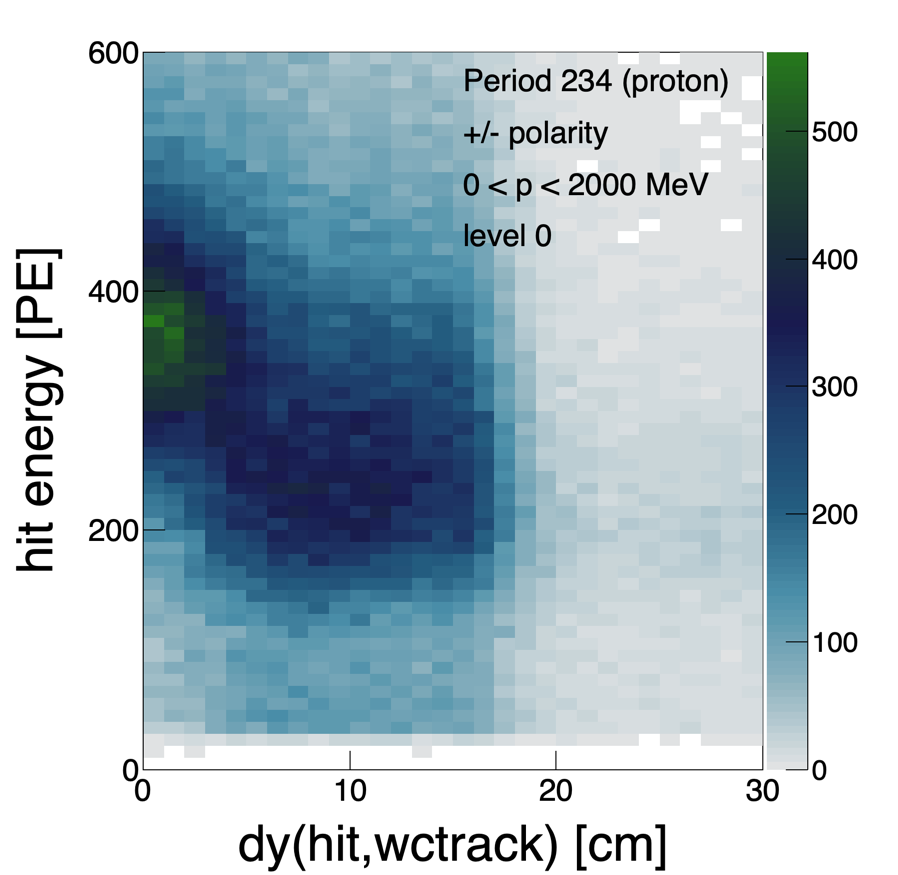
\includegraphics[scale=0.25]{proton_234_hitdy_hitpe_level0_posneg_AllMom_Cur1.png}
     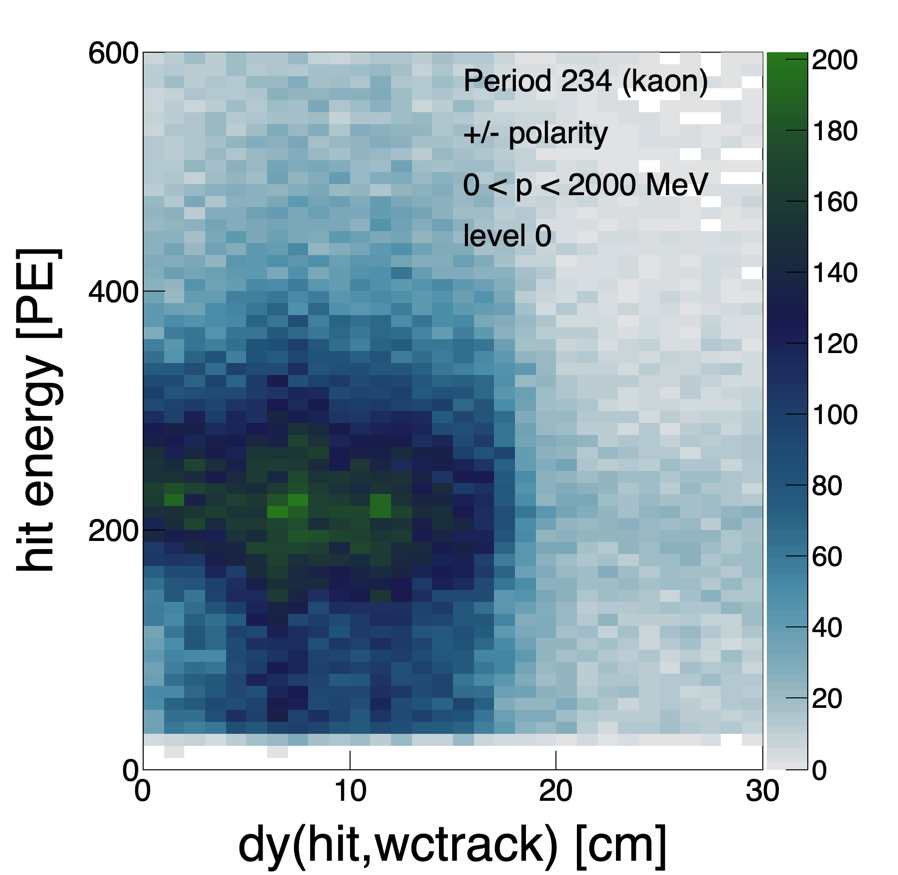
\includegraphics[scale=0.25]{kaon_234_hitdy_hitpe_level0_posneg_AllMom_Cur1.png}
   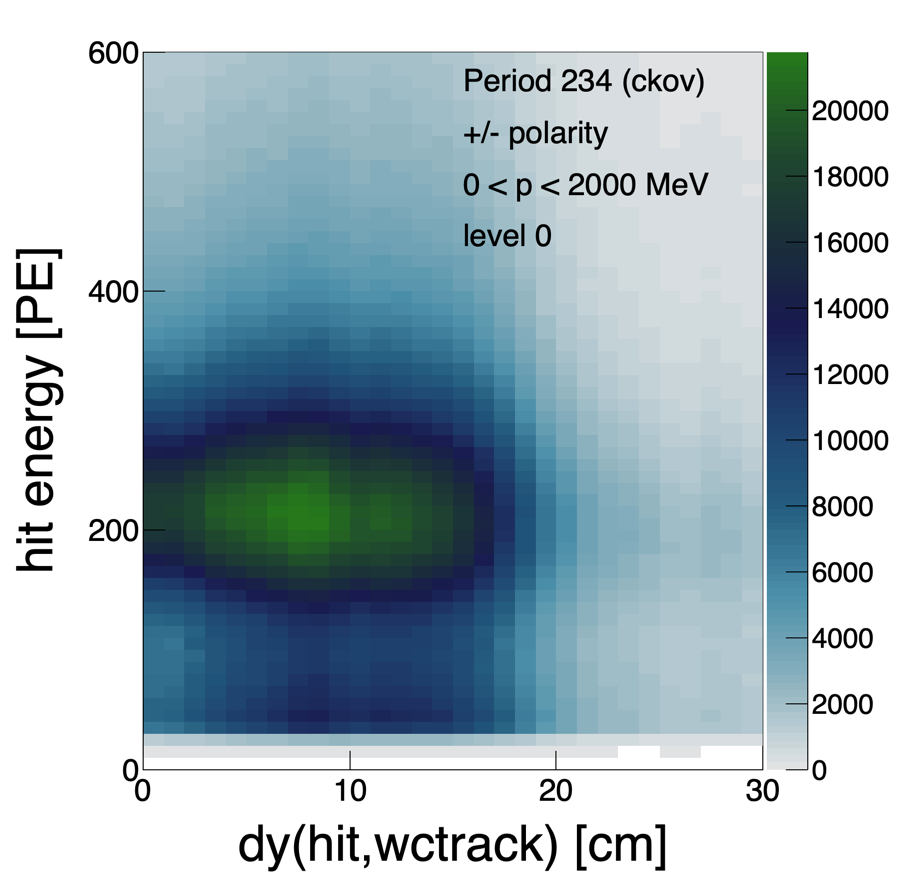
\includegraphics[scale=0.25]{ckov_234_hitdy_hitpe_level0_posneg_AllMom_Cur1.png}
     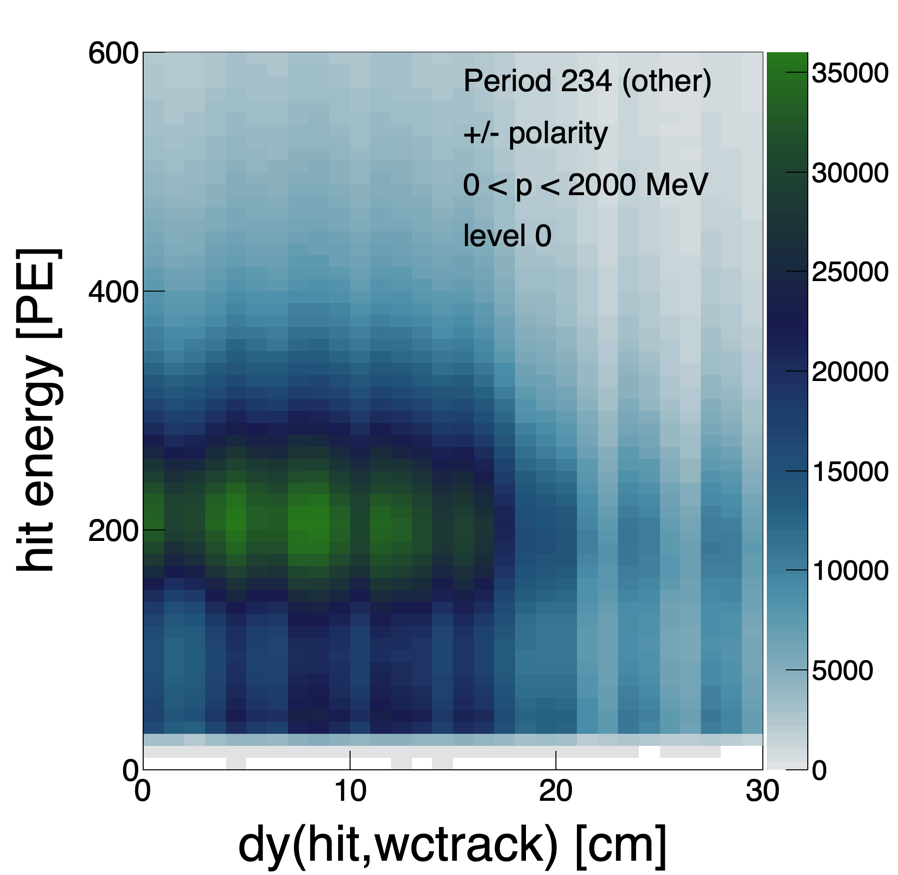
\includegraphics[scale=0.25]{other_234_hitdy_hitpe_level0_posneg_AllMom_Cur1.png}

  \caption{Dy versus PE - script 2d-plot-style.py.}			
   \label{fig_detdype}
  \end{figure}
  
   \begin{figure}	   
 \centering
  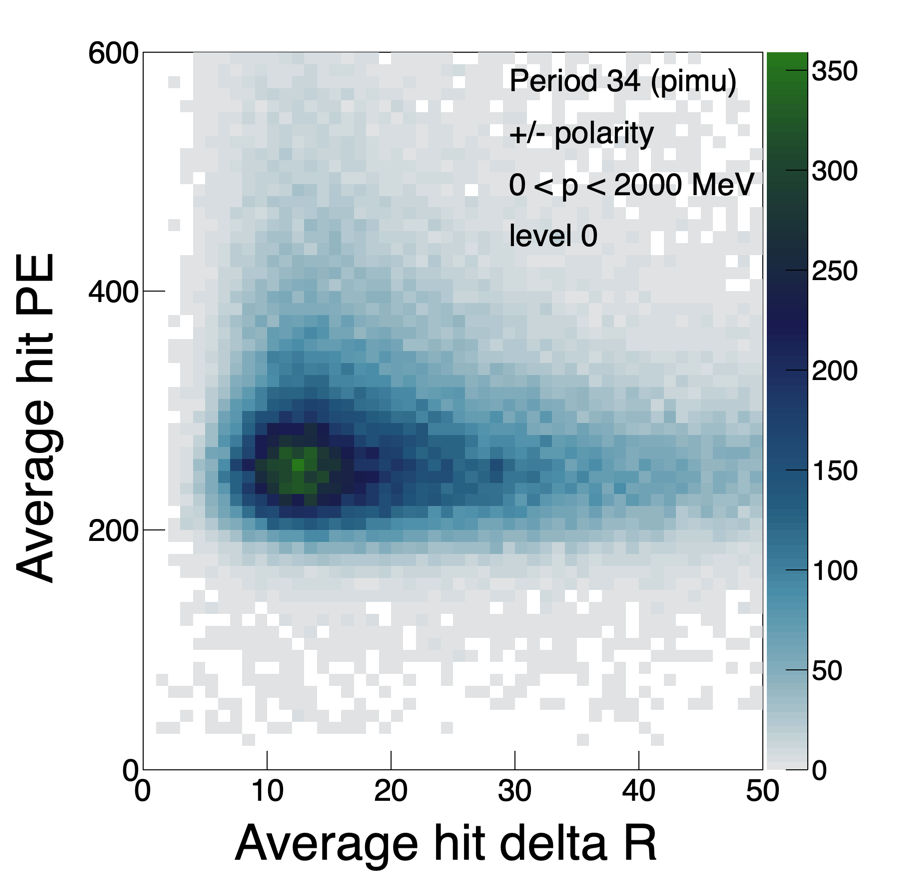
\includegraphics[scale=0.25]{pimu_34_avgdr_avgpe_level0_posneg_AllMom_Cur1.png}
   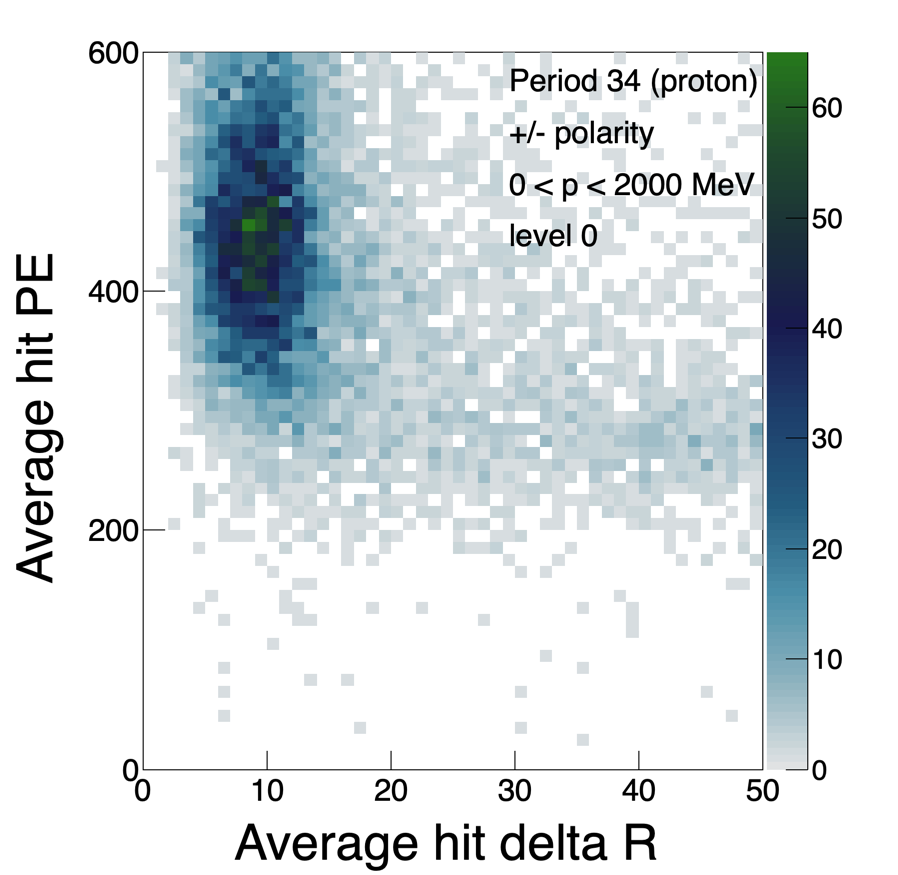
\includegraphics[scale=0.25]{proton_34_avgdr_avgpe_level0_posneg_AllMom_Cur1.png}
     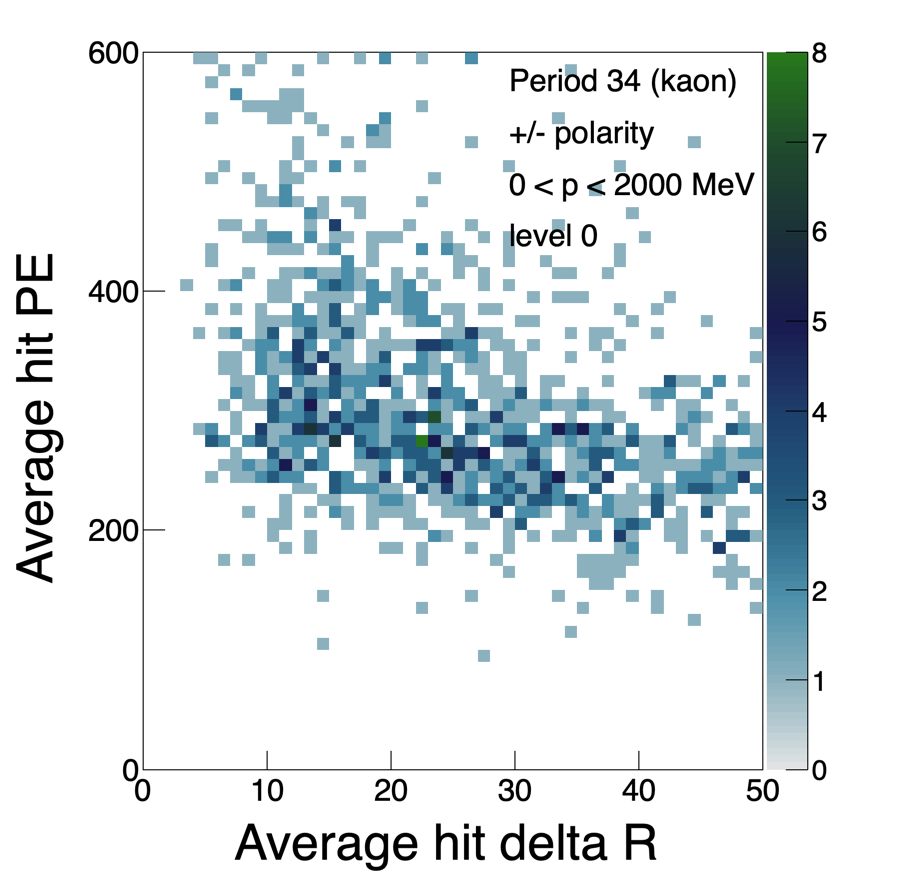
\includegraphics[scale=0.25]{kaon_34_avgdr_avgpe_level0_posneg_AllMom_Cur1.png}
   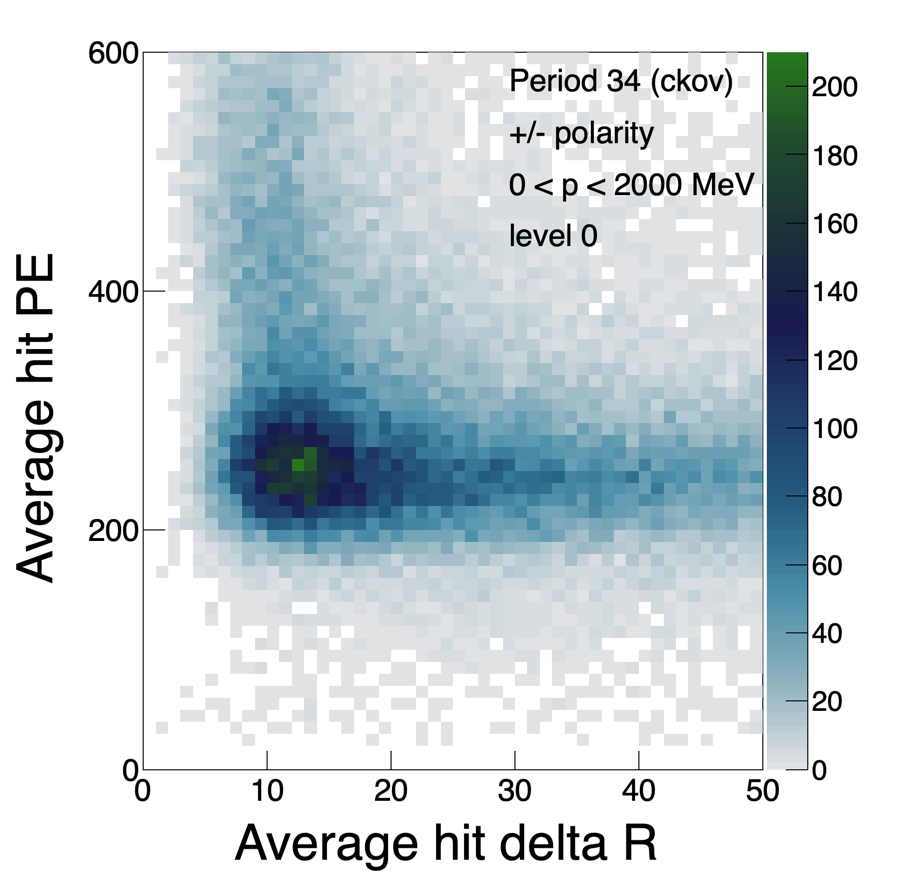
\includegraphics[scale=0.25]{ckov_34_avgdr_avgpe_level0_posneg_AllMom_Cur1.png}
     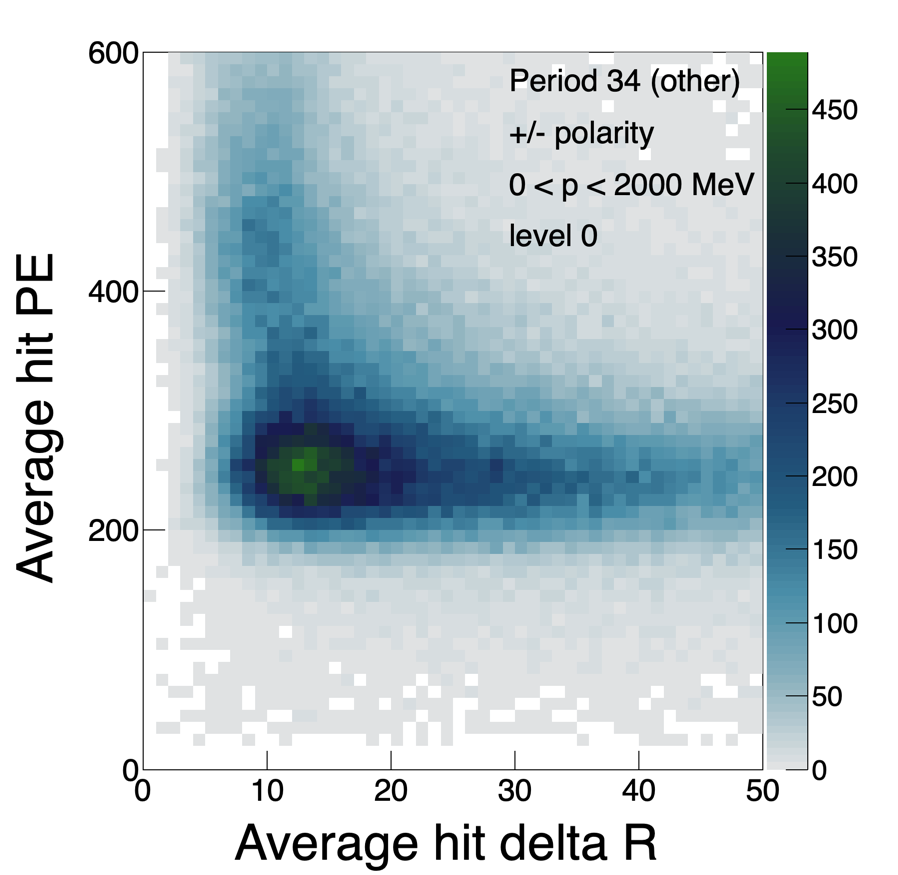
\includegraphics[scale=0.25]{other_34_avgdr_avgpe_level0_posneg_AllMom_Cur1.png}

  \caption{Average Dr versus average PE - script 2d-plot-style.py.}			
   \label{fig_detdrpe}
  \end{figure}

\subsection{Kinetic energy versus last plane with hit}

   \begin{figure}	   
 \centering
  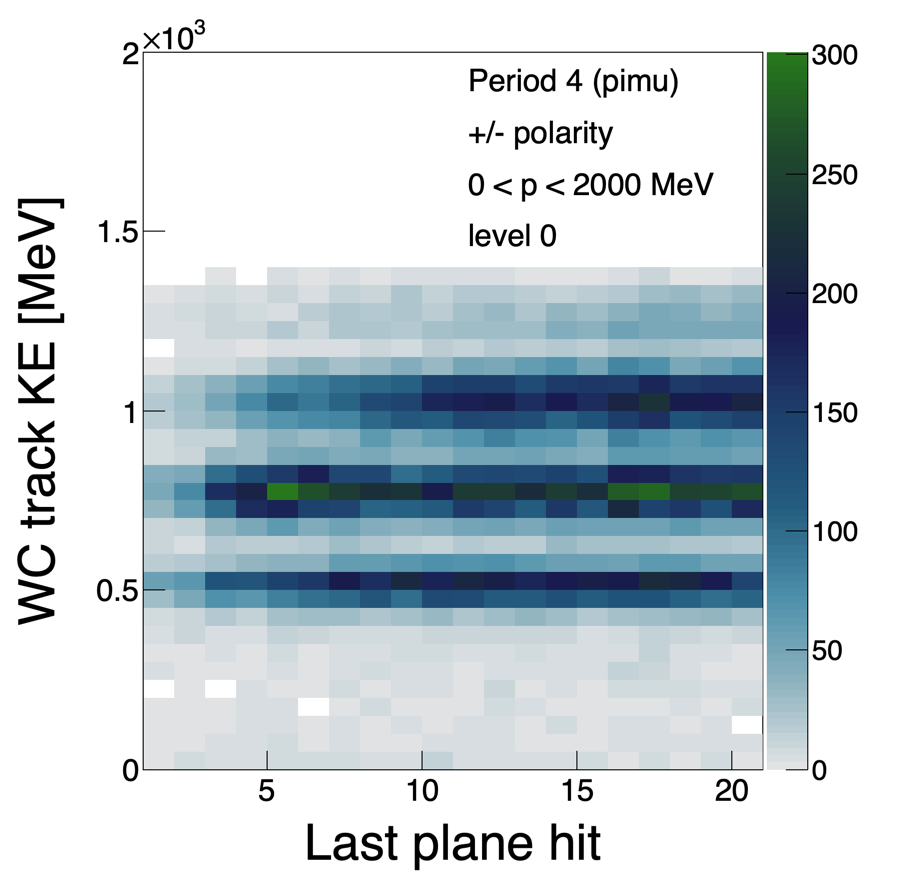
\includegraphics[scale=0.25]{pimu_4_last_ke_level0_posneg_AllMom_Cur1.png}
   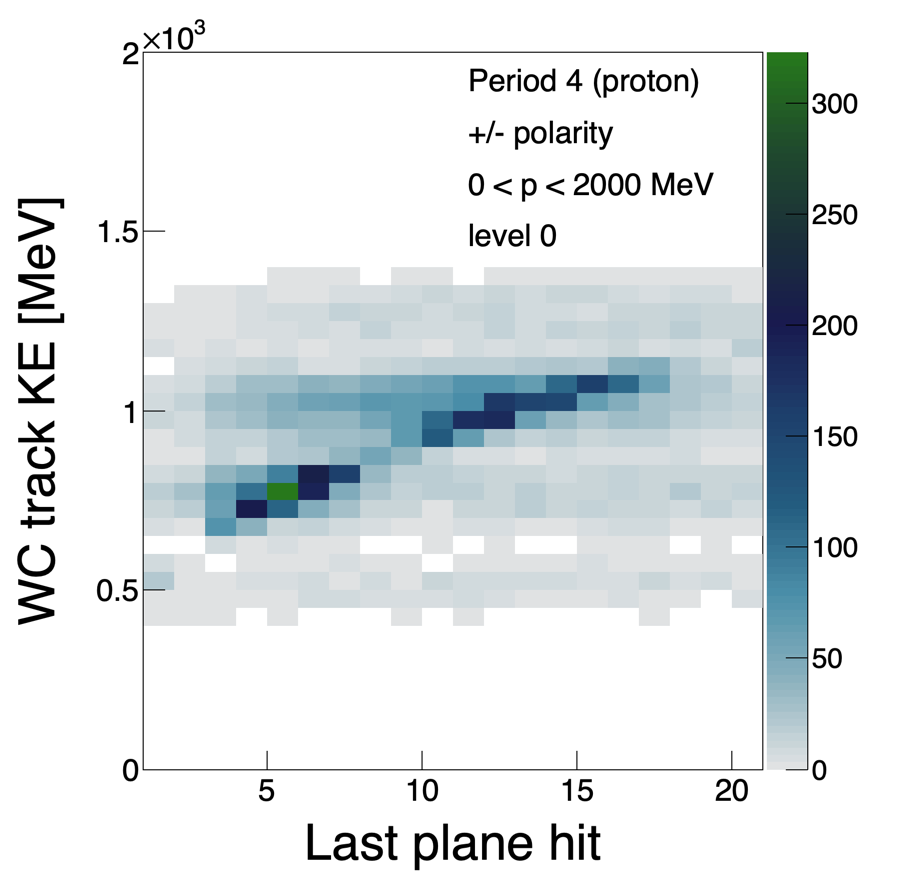
\includegraphics[scale=0.25]{proton_4_last_ke_level0_posneg_AllMom_Cur1.png}
     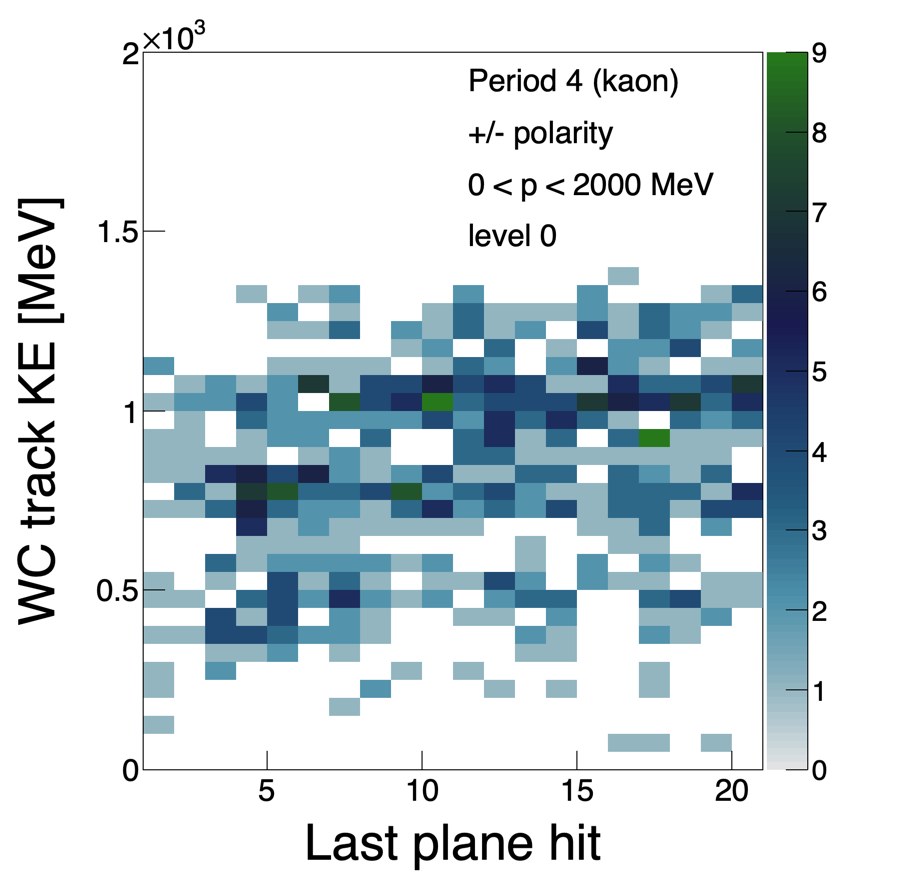
\includegraphics[scale=0.25]{kaon_4_last_ke_level0_posneg_AllMom_Cur1.png}
   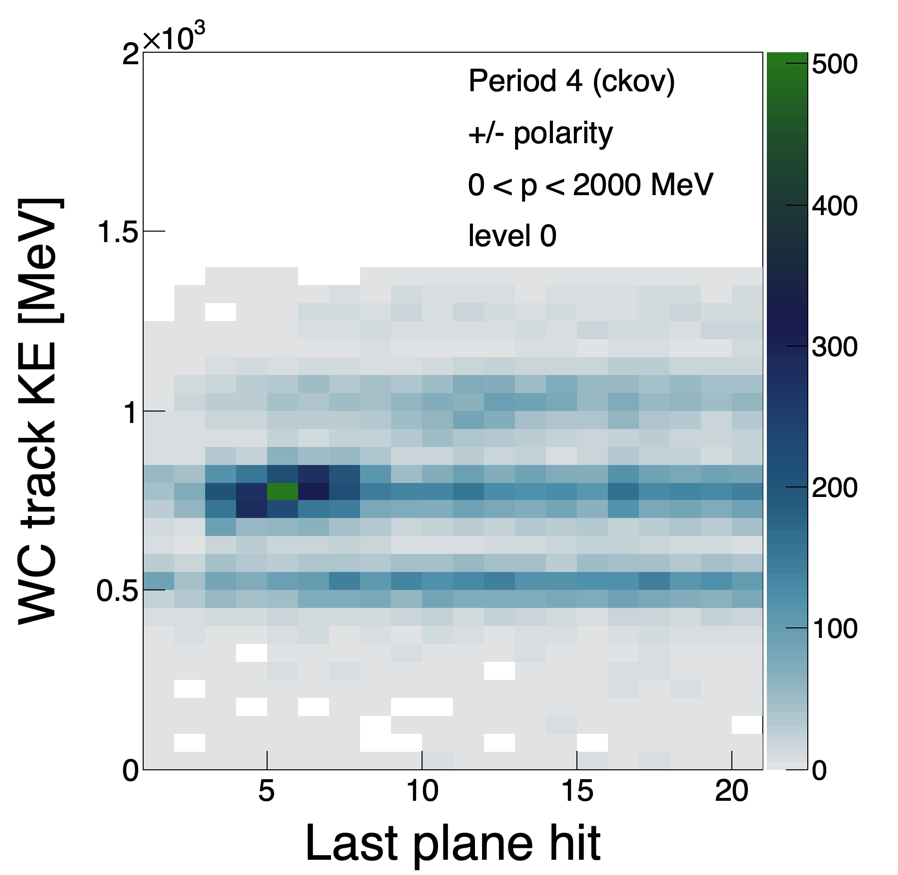
\includegraphics[scale=0.25]{ckov_4_last_ke_level0_posneg_AllMom_Cur1.png}
     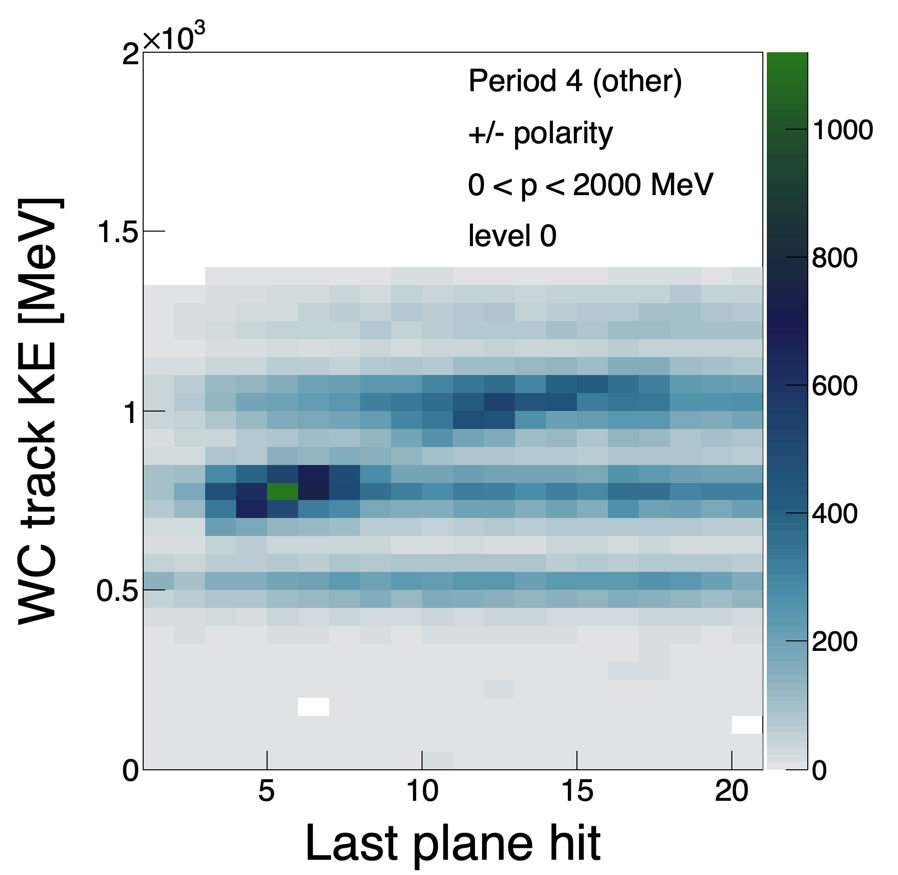
\includegraphics[scale=0.25]{other_4_last_ke_level0_posneg_AllMom_Cur1.png}

  \caption{WC track KE versus last plane containing a hit (limited to planes 1-21) - script 2d-plot-style.py.}			
   \label{fig_detdrpe}
  \end{figure}
  
  
%% DETECTOR PLANE XY PLOTS WITH STRAIGHT LINE FIT
%
\section{All the plots: detector plane rotations}\label{app_fit_XY}

      \begin{figure}[h]	   
 \centering
        	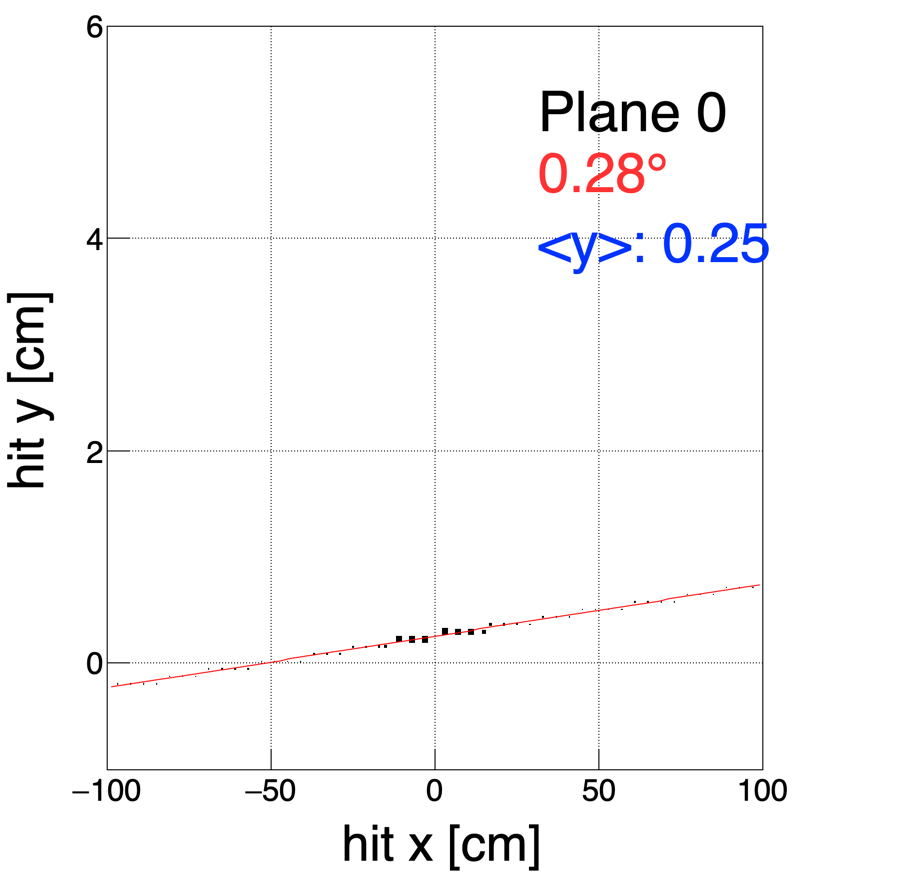
\includegraphics[scale=0.1]{det_xy_pol-1_period4_miss0_plane0.png}
	 	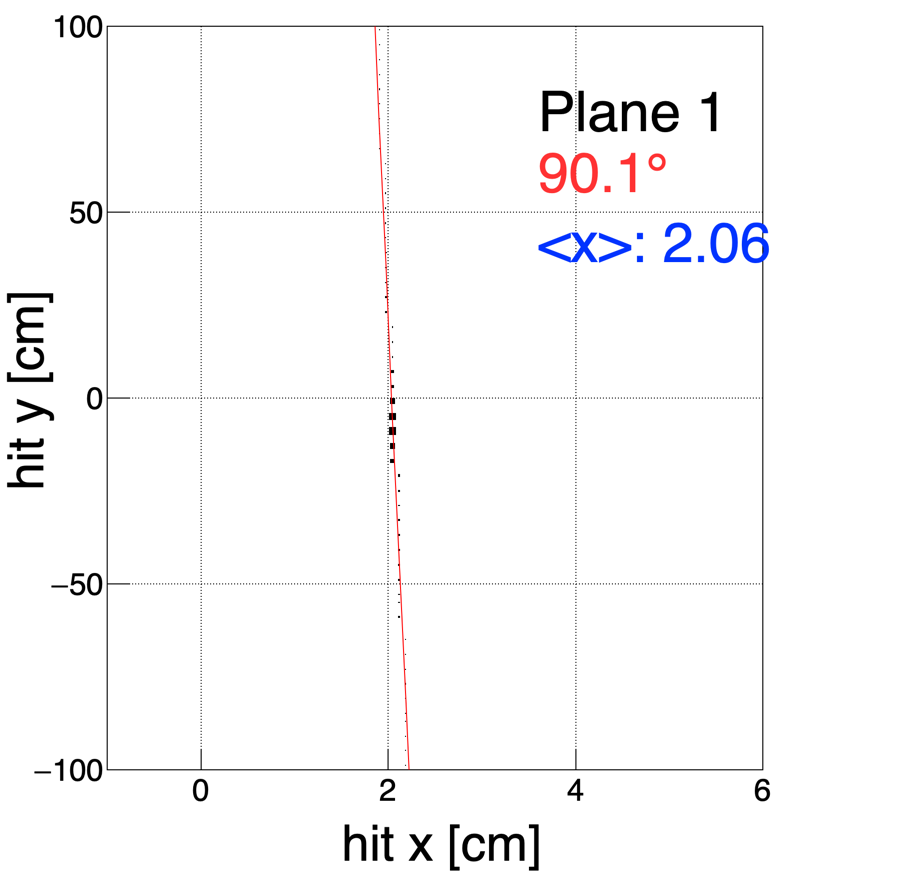
\includegraphics[scale=0.1]{det_xy_pol-1_period4_miss0_plane1.png}
		 	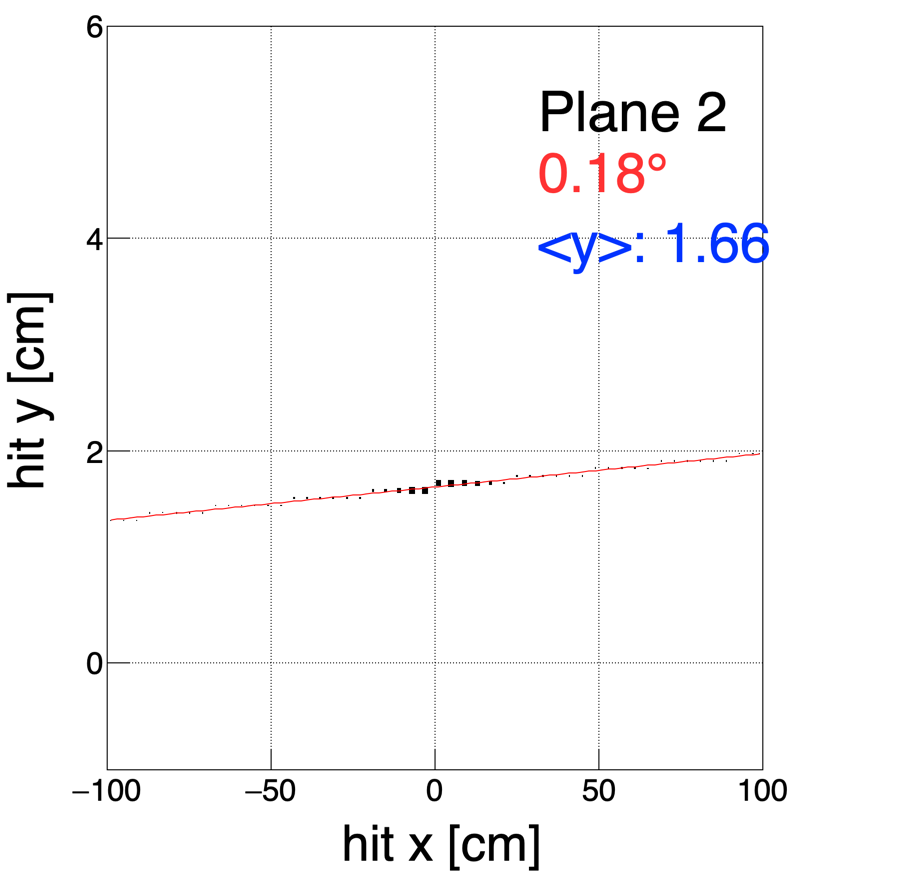
\includegraphics[scale=0.1]{det_xy_pol-1_period4_miss0_plane2.png}
			 	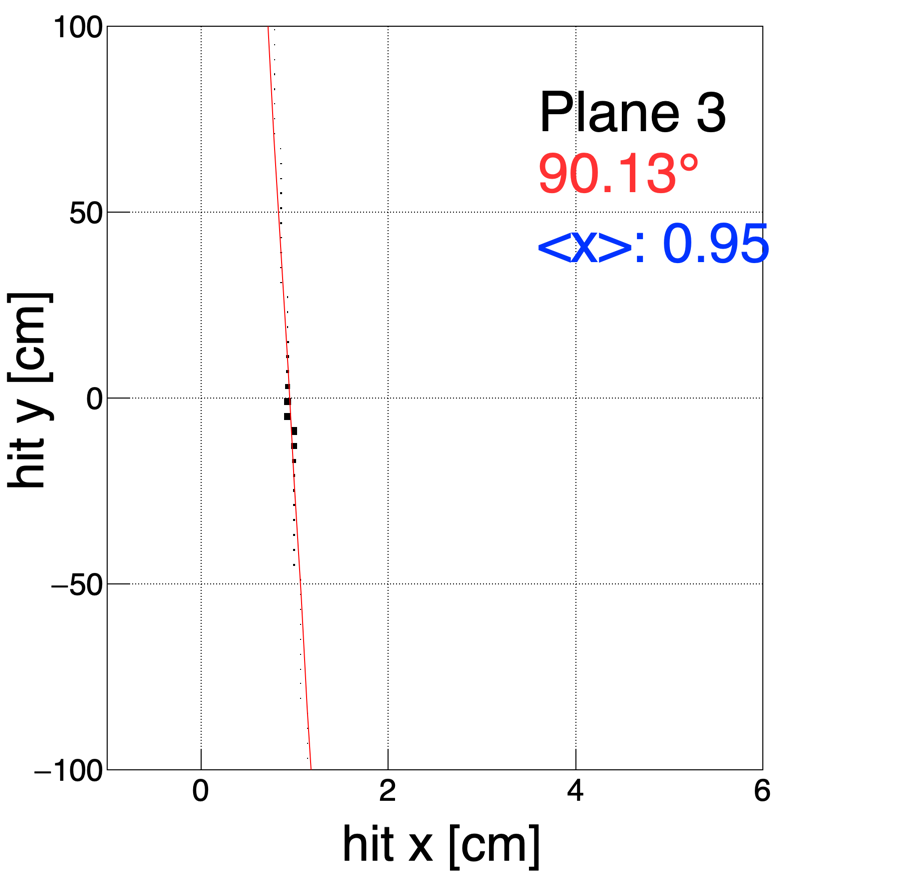
\includegraphics[scale=0.1]{det_xy_pol-1_period4_miss0_plane3.png}
				\includegraphics[scale=0.1]{det_xy_pol-1_period4_miss0_plane4.png}	 
        	\includegraphics[scale=0.1]{det_xy_pol-1_period4_miss0_plane5.png}
	 	\includegraphics[scale=0.1]{det_xy_pol-1_period4_miss0_plane6.png}
		 	\includegraphics[scale=0.1]{det_xy_pol-1_period4_miss0_plane7.png}
			 	\includegraphics[scale=0.1]{det_xy_pol-1_period4_miss0_plane8.png}
				\includegraphics[scale=0.1]{det_xy_pol-1_period4_miss0_plane9.png}					
        	\includegraphics[scale=0.1]{det_xy_pol-1_period4_miss0_plane10.png}
	 	\includegraphics[scale=0.1]{det_xy_pol-1_period4_miss0_plane11.png}
		 	\includegraphics[scale=0.1]{det_xy_pol-1_period4_miss0_plane12.png}
			 	\includegraphics[scale=0.1]{det_xy_pol-1_period4_miss0_plane13.png}
				\includegraphics[scale=0.1]{det_xy_pol-1_period4_miss0_plane14.png}
        	\includegraphics[scale=0.1]{det_xy_pol-1_period4_miss0_plane15.png}
	 	\includegraphics[scale=0.1]{det_xy_pol-1_period4_miss0_plane16.png}
		 	\includegraphics[scale=0.1]{det_xy_pol-1_period4_miss0_plane17.png}
			 	\includegraphics[scale=0.1]{det_xy_pol-1_period4_miss0_plane18.png}
				\includegraphics[scale=0.1]{det_xy_pol-1_period4_miss0_plane19.png}
        	\includegraphics[scale=0.1]{det_xy_pol-1_period4_miss0_plane20.png}
	 	\includegraphics[scale=0.1]{det_xy_pol-1_period4_miss0_plane21.png}
		 	\includegraphics[scale=0.1]{det_xy_pol-1_period4_miss0_plane22.png}
			 	\includegraphics[scale=0.1]{det_xy_pol-1_period4_miss0_plane23.png}
				\includegraphics[scale=0.1]{det_xy_pol-1_period4_miss0_plane24.png}
        	\includegraphics[scale=0.1]{det_xy_pol-1_period4_miss0_plane25.png}
	 	\includegraphics[scale=0.1]{det_xy_pol-1_period4_miss0_plane26.png}
		 	\includegraphics[scale=0.1]{det_xy_pol-1_period4_miss0_plane27.png}
			 	\includegraphics[scale=0.1]{det_xy_pol-1_period4_miss0_plane28.png}
				\includegraphics[scale=0.1]{det_xy_pol-1_period4_miss0_plane29.png}
         	\includegraphics[scale=0.1]{det_xy_pol-1_period4_miss0_plane30.png}
	 	\includegraphics[scale=0.1]{det_xy_pol-1_period4_miss0_plane31.png}
		 	\includegraphics[scale=0.1]{det_xy_pol-1_period4_miss0_plane32.png}
			 	\includegraphics[scale=0.1]{det_xy_pol-1_period4_miss0_plane33.png}
				\includegraphics[scale=0.1]{det_xy_pol-1_period4_miss0_plane34.png}
   \caption[short]{Detector hit positions by plane for the first 35 planes.}
   \label{fig_dethit_first35}
  \end{figure}
  
  
        \begin{figure}[h]	   
 \centering
        	\includegraphics[scale=0.1]{det_xy_pol-1_period4_miss0_plane35.png}
	 	\includegraphics[scale=0.1]{det_xy_pol-1_period4_miss0_plane36.png}
		 	\includegraphics[scale=0.1]{det_xy_pol-1_period4_miss0_plane37.png}
			 	\includegraphics[scale=0.1]{det_xy_pol-1_period4_miss0_plane38.png}
				\includegraphics[scale=0.1]{det_xy_pol-1_period4_miss0_plane39.png}	 
        	\includegraphics[scale=0.1]{det_xy_pol-1_period4_miss0_plane40.png}
	 	\includegraphics[scale=0.1]{det_xy_pol-1_period4_miss0_plane41.png}
		 	\includegraphics[scale=0.1]{det_xy_pol-1_period4_miss0_plane42.png}
			 	\includegraphics[scale=0.1]{det_xy_pol-1_period4_miss0_plane43.png}
				\includegraphics[scale=0.1]{det_xy_pol-1_period4_miss0_plane44.png}					
        	\includegraphics[scale=0.1]{det_xy_pol-1_period4_miss0_plane45.png}
	 	\includegraphics[scale=0.1]{det_xy_pol-1_period4_miss0_plane46.png}
		 	\includegraphics[scale=0.1]{det_xy_pol-1_period4_miss0_plane47.png}
			 	\includegraphics[scale=0.1]{det_xy_pol-1_period4_miss0_plane48.png}
				\includegraphics[scale=0.1]{det_xy_pol-1_period4_miss0_plane49.png}
        	\includegraphics[scale=0.1]{det_xy_pol-1_period4_miss0_plane50.png}
	 	\includegraphics[scale=0.1]{det_xy_pol-1_period4_miss0_plane51.png}
		 	\includegraphics[scale=0.1]{det_xy_pol-1_period4_miss0_plane52.png}
			 	\includegraphics[scale=0.1]{det_xy_pol-1_period4_miss0_plane53.png}
				\includegraphics[scale=0.1]{det_xy_pol-1_period4_miss0_plane54.png}
        	\includegraphics[scale=0.1]{det_xy_pol-1_period4_miss0_plane55.png}
	 	\includegraphics[scale=0.1]{det_xy_pol-1_period4_miss0_plane56.png}
		 	\includegraphics[scale=0.1]{det_xy_pol-1_period4_miss0_plane57.png}
			 	\includegraphics[scale=0.1]{det_xy_pol-1_period4_miss0_plane58.png}
				\includegraphics[scale=0.1]{det_xy_pol-1_period4_miss0_plane59.png}
        	\includegraphics[scale=0.1]{det_xy_pol-1_period4_miss0_plane60.png}
	 	\includegraphics[scale=0.1]{det_xy_pol-1_period4_miss0_plane61.png}
		 	\includegraphics[scale=0.1]{det_xy_pol-1_period4_miss0_plane62.png}
\caption{Detector hit positions in planes 35-62}			
   \label{fig_dethit_last}
  \end{figure}
  
  
  
  
% DETECTOR PLANE ENERGY XY PLOTS PE AND GEV

  \section{All the plots: Energy versus x/y}\label{app_PE_XY}
  
  
  Detector hit PE as a function of x(y) in vertical (horizontal) planes are show in Figures~\ref{fig_detxpe_first} and ~\ref{fig_detxpe_last}. Plots made using the script \texttt{single-plot-detxpe.py}.
  
        \begin{figure}[h]	   
 \centering
        	\includegraphics[scale=0.1]{det_xype_pol-1_period4_miss0_plane0.png}
	 	\includegraphics[scale=0.1]{det_xype_pol-1_period4_miss0_plane1.png}
		 	\includegraphics[scale=0.1]{det_xype_pol-1_period4_miss0_plane2.png}
			 	\includegraphics[scale=0.1]{det_xype_pol-1_period4_miss0_plane3.png}
				\includegraphics[scale=0.1]{det_xype_pol-1_period4_miss0_plane4.png}	 
        	\includegraphics[scale=0.1]{det_xype_pol-1_period4_miss0_plane5.png}
	 	\includegraphics[scale=0.1]{det_xype_pol-1_period4_miss0_plane6.png}
		 	\includegraphics[scale=0.1]{det_xype_pol-1_period4_miss0_plane7.png}
			 	\includegraphics[scale=0.1]{det_xype_pol-1_period4_miss0_plane8.png}
				\includegraphics[scale=0.1]{det_xype_pol-1_period4_miss0_plane9.png}					
        	\includegraphics[scale=0.1]{det_xype_pol-1_period4_miss0_plane10.png}
	 	\includegraphics[scale=0.1]{det_xype_pol-1_period4_miss0_plane11.png}
		 	\includegraphics[scale=0.1]{det_xype_pol-1_period4_miss0_plane12.png}
			 	\includegraphics[scale=0.1]{det_xype_pol-1_period4_miss0_plane13.png}
				\includegraphics[scale=0.1]{det_xype_pol-1_period4_miss0_plane14.png}
        	\includegraphics[scale=0.1]{det_xype_pol-1_period4_miss0_plane15.png}
	 	\includegraphics[scale=0.1]{det_xype_pol-1_period4_miss0_plane16.png}
		 	\includegraphics[scale=0.1]{det_xype_pol-1_period4_miss0_plane17.png}
			 	\includegraphics[scale=0.1]{det_xype_pol-1_period4_miss0_plane18.png}
				\includegraphics[scale=0.1]{det_xype_pol-1_period4_miss0_plane19.png}
        	\includegraphics[scale=0.1]{det_xype_pol-1_period4_miss0_plane20.png}
	 	\includegraphics[scale=0.1]{det_xype_pol-1_period4_miss0_plane21.png}
		 	\includegraphics[scale=0.1]{det_xype_pol-1_period4_miss0_plane22.png}
			 	\includegraphics[scale=0.1]{det_xype_pol-1_period4_miss0_plane23.png}
				\includegraphics[scale=0.1]{det_xype_pol-1_period4_miss0_plane24.png}
        	\includegraphics[scale=0.1]{det_xype_pol-1_period4_miss0_plane25.png}
	 	\includegraphics[scale=0.1]{det_xype_pol-1_period4_miss0_plane26.png}
		 	\includegraphics[scale=0.1]{det_xype_pol-1_period4_miss0_plane27.png}
			 	\includegraphics[scale=0.1]{det_xype_pol-1_period4_miss0_plane28.png}
				\includegraphics[scale=0.1]{det_xype_pol-1_period4_miss0_plane29.png}
         	\includegraphics[scale=0.1]{det_xype_pol-1_period4_miss0_plane30.png}
	 	\includegraphics[scale=0.1]{det_xype_pol-1_period4_miss0_plane31.png}
		 	\includegraphics[scale=0.1]{det_xype_pol-1_period4_miss0_plane32.png}
			 	\includegraphics[scale=0.1]{det_xype_pol-1_period4_miss0_plane33.png}
				\includegraphics[scale=0.1]{det_xype_pol-1_period4_miss0_plane34.png}
   \caption[short]{Detector CellHit PE by plane for the first 35 planes.}
   \label{fig_detxpe_first}
  \end{figure}
  
  
        \begin{figure}[h]	   
 \centering
        	\includegraphics[scale=0.1]{det_xype_pol-1_period4_miss0_plane35.png}
	 	\includegraphics[scale=0.1]{det_xype_pol-1_period4_miss0_plane36.png}
		 	\includegraphics[scale=0.1]{det_xype_pol-1_period4_miss0_plane37.png}
			 	\includegraphics[scale=0.1]{det_xype_pol-1_period4_miss0_plane38.png}
				\includegraphics[scale=0.1]{det_xype_pol-1_period4_miss0_plane39.png}	 
        	\includegraphics[scale=0.1]{det_xype_pol-1_period4_miss0_plane40.png}
	 	\includegraphics[scale=0.1]{det_xype_pol-1_period4_miss0_plane41.png}
		 	\includegraphics[scale=0.1]{det_xype_pol-1_period4_miss0_plane42.png}
			 	\includegraphics[scale=0.1]{det_xype_pol-1_period4_miss0_plane43.png}
				\includegraphics[scale=0.1]{det_xype_pol-1_period4_miss0_plane44.png}					
        	\includegraphics[scale=0.1]{det_xype_pol-1_period4_miss0_plane45.png}
	 	\includegraphics[scale=0.1]{det_xype_pol-1_period4_miss0_plane46.png}
		 	\includegraphics[scale=0.1]{det_xype_pol-1_period4_miss0_plane47.png}
			 	\includegraphics[scale=0.1]{det_xype_pol-1_period4_miss0_plane48.png}
				\includegraphics[scale=0.1]{det_xype_pol-1_period4_miss0_plane49.png}
        	\includegraphics[scale=0.1]{det_xype_pol-1_period4_miss0_plane50.png}
	 	\includegraphics[scale=0.1]{det_xype_pol-1_period4_miss0_plane51.png}
		 	\includegraphics[scale=0.1]{det_xype_pol-1_period4_miss0_plane52.png}
			 	\includegraphics[scale=0.1]{det_xype_pol-1_period4_miss0_plane53.png}
				\includegraphics[scale=0.1]{det_xype_pol-1_period4_miss0_plane54.png}
        	\includegraphics[scale=0.1]{det_xype_pol-1_period4_miss0_plane55.png}
	 	\includegraphics[scale=0.1]{det_xype_pol-1_period4_miss0_plane56.png}
		 	\includegraphics[scale=0.1]{det_xype_pol-1_period4_miss0_plane57.png}
			 	\includegraphics[scale=0.1]{det_xype_pol-1_period4_miss0_plane58.png}
				\includegraphics[scale=0.1]{det_xype_pol-1_period4_miss0_plane59.png}
        	\includegraphics[scale=0.1]{det_xype_pol-1_period4_miss0_plane60.png}
	 	\includegraphics[scale=0.1]{det_xype_pol-1_period4_miss0_plane61.png}
		 	\includegraphics[scale=0.1]{det_xype_pol-1_period4_miss0_plane62.png}
\caption{Detector CellHit PE in planes 35-62}			
   \label{fig_detxpe_last}
  \end{figure}

Detector hit GeV as a function of x(y) in vertical (horizontal) planes are show in Figures~\ref{fig_detxgev_first} and ~\ref{fig_detxgev_last}. Plots made using the script \texttt{single-plot-detxgev.py}.
  
        \begin{figure}[h]	   
 \centering
        	\includegraphics[scale=0.1]{det_xygev_pol-1_period4_miss0_plane0.png}
	 	\includegraphics[scale=0.1]{det_xygev_pol-1_period4_miss0_plane1.png}
		 	\includegraphics[scale=0.1]{det_xygev_pol-1_period4_miss0_plane2.png}
			 	\includegraphics[scale=0.1]{det_xygev_pol-1_period4_miss0_plane3.png}
				\includegraphics[scale=0.1]{det_xygev_pol-1_period4_miss0_plane4.png}	 
        	\includegraphics[scale=0.1]{det_xygev_pol-1_period4_miss0_plane5.png}
	 	\includegraphics[scale=0.1]{det_xygev_pol-1_period4_miss0_plane6.png}
		 	\includegraphics[scale=0.1]{det_xygev_pol-1_period4_miss0_plane7.png}
			 	\includegraphics[scale=0.1]{det_xygev_pol-1_period4_miss0_plane8.png}
				\includegraphics[scale=0.1]{det_xygev_pol-1_period4_miss0_plane9.png}					
        	\includegraphics[scale=0.1]{det_xygev_pol-1_period4_miss0_plane10.png}
	 	\includegraphics[scale=0.1]{det_xygev_pol-1_period4_miss0_plane11.png}
		 	\includegraphics[scale=0.1]{det_xygev_pol-1_period4_miss0_plane12.png}
			 	\includegraphics[scale=0.1]{det_xygev_pol-1_period4_miss0_plane13.png}
				\includegraphics[scale=0.1]{det_xygev_pol-1_period4_miss0_plane14.png}
        	\includegraphics[scale=0.1]{det_xygev_pol-1_period4_miss0_plane15.png}
	 	\includegraphics[scale=0.1]{det_xygev_pol-1_period4_miss0_plane16.png}
		 	\includegraphics[scale=0.1]{det_xygev_pol-1_period4_miss0_plane17.png}
			 	\includegraphics[scale=0.1]{det_xygev_pol-1_period4_miss0_plane18.png}
				\includegraphics[scale=0.1]{det_xygev_pol-1_period4_miss0_plane19.png}
        	\includegraphics[scale=0.1]{det_xygev_pol-1_period4_miss0_plane20.png}
	 	\includegraphics[scale=0.1]{det_xygev_pol-1_period4_miss0_plane21.png}
		 	\includegraphics[scale=0.1]{det_xygev_pol-1_period4_miss0_plane22.png}
			 	\includegraphics[scale=0.1]{det_xygev_pol-1_period4_miss0_plane23.png}
				\includegraphics[scale=0.1]{det_xygev_pol-1_period4_miss0_plane24.png}
        	\includegraphics[scale=0.1]{det_xygev_pol-1_period4_miss0_plane25.png}
	 	\includegraphics[scale=0.1]{det_xygev_pol-1_period4_miss0_plane26.png}
		 	\includegraphics[scale=0.1]{det_xygev_pol-1_period4_miss0_plane27.png}
			 	\includegraphics[scale=0.1]{det_xygev_pol-1_period4_miss0_plane28.png}
				\includegraphics[scale=0.1]{det_xygev_pol-1_period4_miss0_plane29.png}
         	\includegraphics[scale=0.1]{det_xygev_pol-1_period4_miss0_plane30.png}
	 	\includegraphics[scale=0.1]{det_xygev_pol-1_period4_miss0_plane31.png}
		 	\includegraphics[scale=0.1]{det_xygev_pol-1_period4_miss0_plane32.png}
			 	\includegraphics[scale=0.1]{det_xygev_pol-1_period4_miss0_plane33.png}
				\includegraphics[scale=0.1]{det_xygev_pol-1_period4_miss0_plane34.png}
   \caption[short]{Detector CellHit calibrated energy aka GeV in the first 35 planes.}
   \label{fig_detxgev_first}
  \end{figure}
  
  
        \begin{figure}[h]	   
 \centering
        	\includegraphics[scale=0.1]{det_xygev_pol-1_period4_miss0_plane35.png}
	 	\includegraphics[scale=0.1]{det_xygev_pol-1_period4_miss0_plane36.png}
		 	\includegraphics[scale=0.1]{det_xygev_pol-1_period4_miss0_plane37.png}
			 	\includegraphics[scale=0.1]{det_xygev_pol-1_period4_miss0_plane38.png}
				\includegraphics[scale=0.1]{det_xygev_pol-1_period4_miss0_plane39.png}	 
        	\includegraphics[scale=0.1]{det_xygev_pol-1_period4_miss0_plane40.png}
	 	\includegraphics[scale=0.1]{det_xygev_pol-1_period4_miss0_plane41.png}
		 	\includegraphics[scale=0.1]{det_xygev_pol-1_period4_miss0_plane42.png}
			 	\includegraphics[scale=0.1]{det_xygev_pol-1_period4_miss0_plane43.png}
				\includegraphics[scale=0.1]{det_xygev_pol-1_period4_miss0_plane44.png}					
        	\includegraphics[scale=0.1]{det_xygev_pol-1_period4_miss0_plane45.png}
	 	\includegraphics[scale=0.1]{det_xygev_pol-1_period4_miss0_plane46.png}
		 	\includegraphics[scale=0.1]{det_xygev_pol-1_period4_miss0_plane47.png}
			 	\includegraphics[scale=0.1]{det_xygev_pol-1_period4_miss0_plane48.png}
				\includegraphics[scale=0.1]{det_xygev_pol-1_period4_miss0_plane49.png}
        	\includegraphics[scale=0.1]{det_xygev_pol-1_period4_miss0_plane50.png}
	 	\includegraphics[scale=0.1]{det_xygev_pol-1_period4_miss0_plane51.png}
		 	\includegraphics[scale=0.1]{det_xygev_pol-1_period4_miss0_plane52.png}
			 	\includegraphics[scale=0.1]{det_xygev_pol-1_period4_miss0_plane53.png}
				\includegraphics[scale=0.1]{det_xygev_pol-1_period4_miss0_plane54.png}
        	\includegraphics[scale=0.1]{det_xygev_pol-1_period4_miss0_plane55.png}
	 	\includegraphics[scale=0.1]{det_xygev_pol-1_period4_miss0_plane56.png}
		 	\includegraphics[scale=0.1]{det_xygev_pol-1_period4_miss0_plane57.png}
			 	\includegraphics[scale=0.1]{det_xygev_pol-1_period4_miss0_plane58.png}
				\includegraphics[scale=0.1]{det_xygev_pol-1_period4_miss0_plane59.png}
        	\includegraphics[scale=0.1]{det_xygev_pol-1_period4_miss0_plane60.png}
	 	\includegraphics[scale=0.1]{det_xygev_pol-1_period4_miss0_plane61.png}
		 	\includegraphics[scale=0.1]{det_xygev_pol-1_period4_miss0_plane62.png}
\caption{Detector CellHit calibrated energy aka GeV in planes 35-62}			
   \label{fig_detxgev_last}
  \end{figure}

\end{document}